\chapter[Detailed Design]{Chapter 4: Detailed Design}\label{chap:hard_dsgn}%This chapter must be a lot of pages.
%*******************************************%
\section{Introduction}\label{sec:intro_dsgn}
%*******************************************%
In this chapter, we delve into the comprehensive design process for the proposed scalable modular Battery Management System. Initially, the design processes for the independent monitoring modules and the main controller are explored separately. Subsequently, the communication system combines the designs of these entities as the main controller serves to collect and process the data monitored by the cell modules. The systematic approach for the design process entails the circuit designs, component selection, and the printed circuit board layout. Afterwards a merged design review of the system is done.
%*******************************************%
\section{System Overview}\label{subsec:syst_OVV}
%########################################################
As illustrated in figure \ref{fig:ovvv_dsgn} below the modular BMS design essentially has the same setup as a traditional BMS but the whole system is fitted to each cell independently. As a result, every cell in the series string is equipped with a monitoring module connected in parallel, enabling us to acquire more accurate and precise measurements from each cell. These modules feature their own microcontroller, responsible for processing the measurements and transferring the data to a master device for storage or sharing. Additionally, all the boards are interconnected, allowing for seamless communication and establishing a global view of the battery pack. This collective understanding enables each module to assess the state of the entire pack and make necessary adjustments to its respective cell’s variables.

\begin{figure}[h!]
\centering
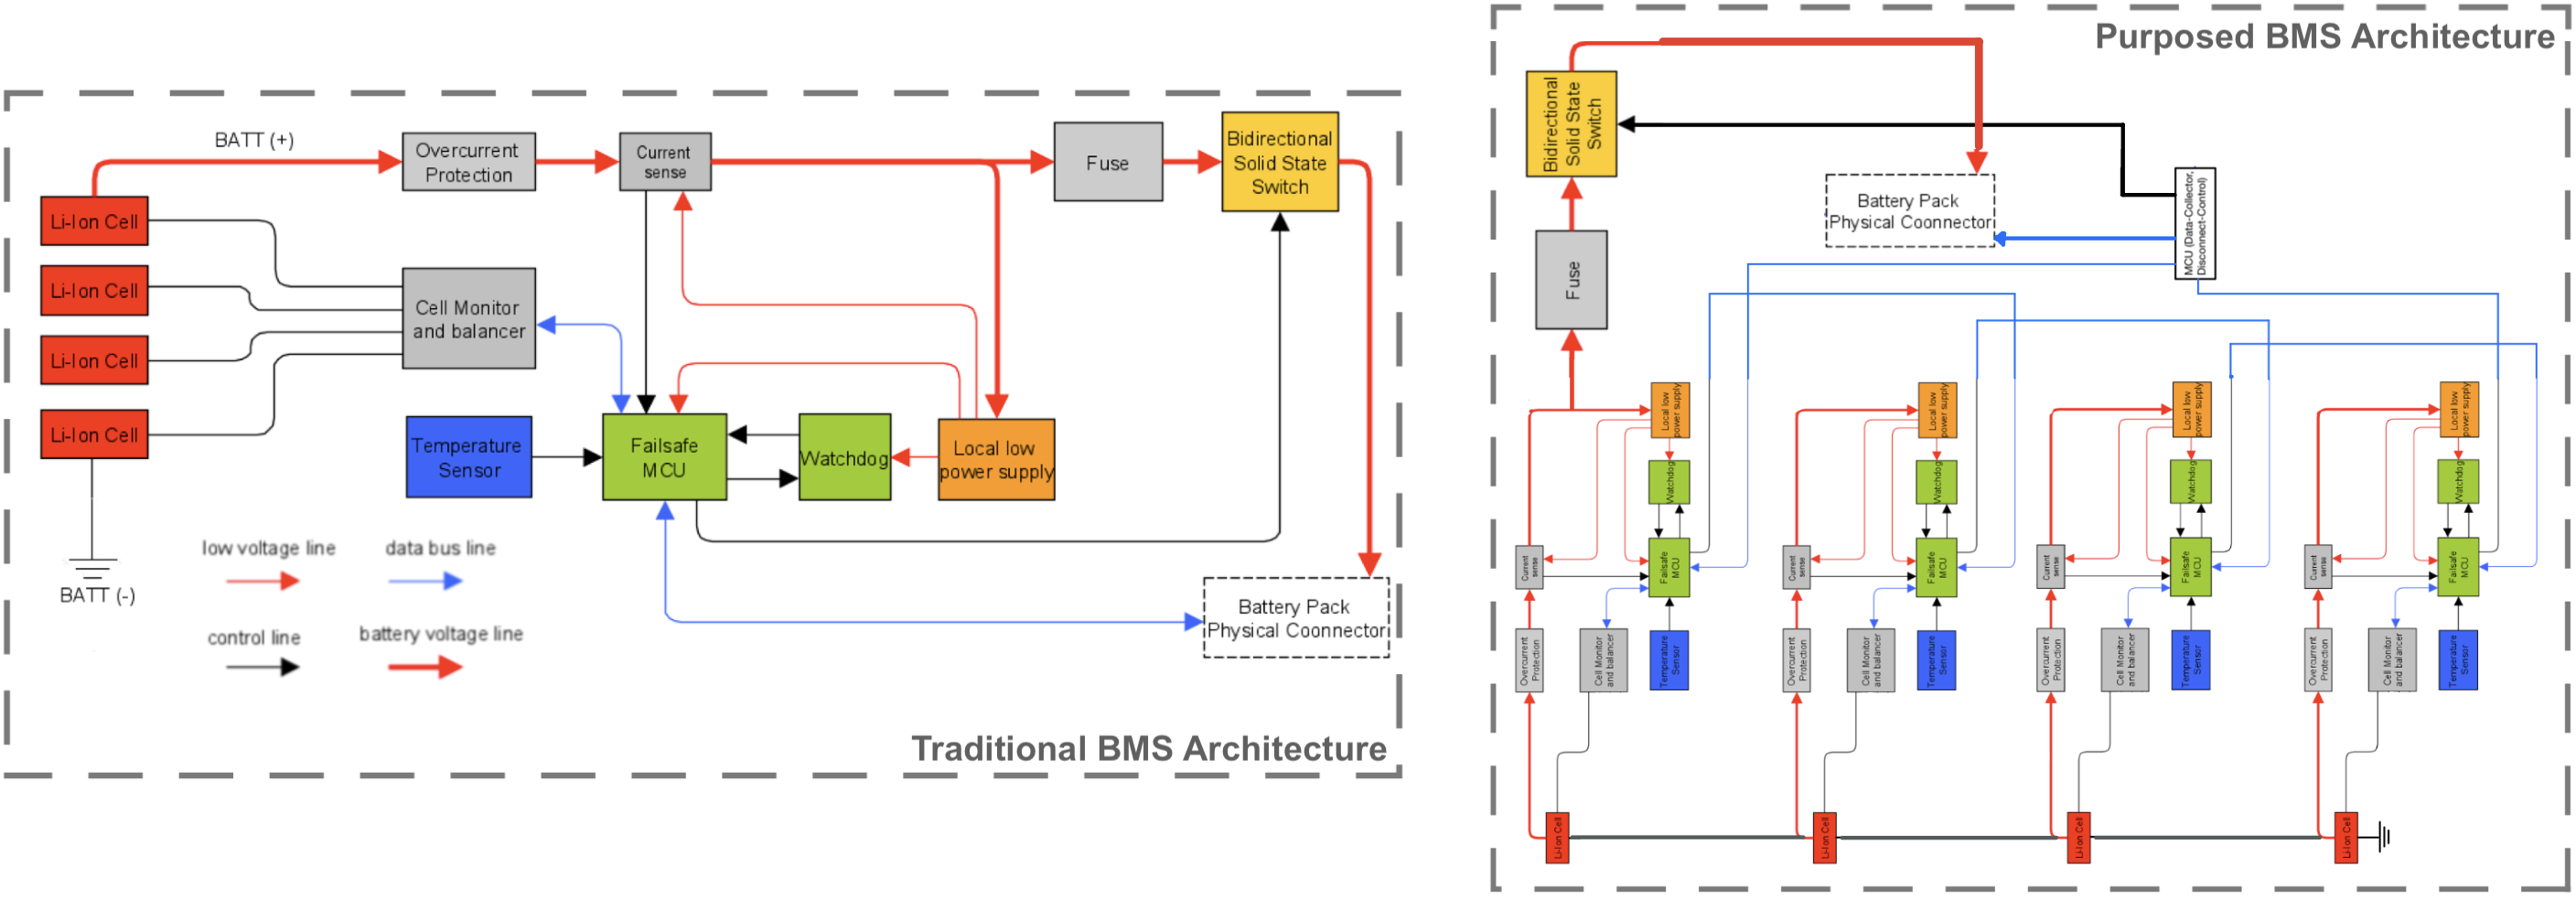
\includegraphics[width=0.9\textwidth]{Skripsie_LaTeXTemplate/Figures/simpleBMS_Diagram.png}
\caption{Envisioned Architecture of the Proposed BMS}
\label{fig:ovvv_dsgn}
\end{figure}

\noindent
The BMS monitoring boards will be attached to each cell in the battery pack. Their sole wired connection will be the communication line linking the cells, which significantly reduces the use of extensive wiring in the system. The primary (master) controller, located externally, interfaces with the battery pack and facilitates connections to either the load or charger.
\newpage
\begin{figure}[h!]
\centering
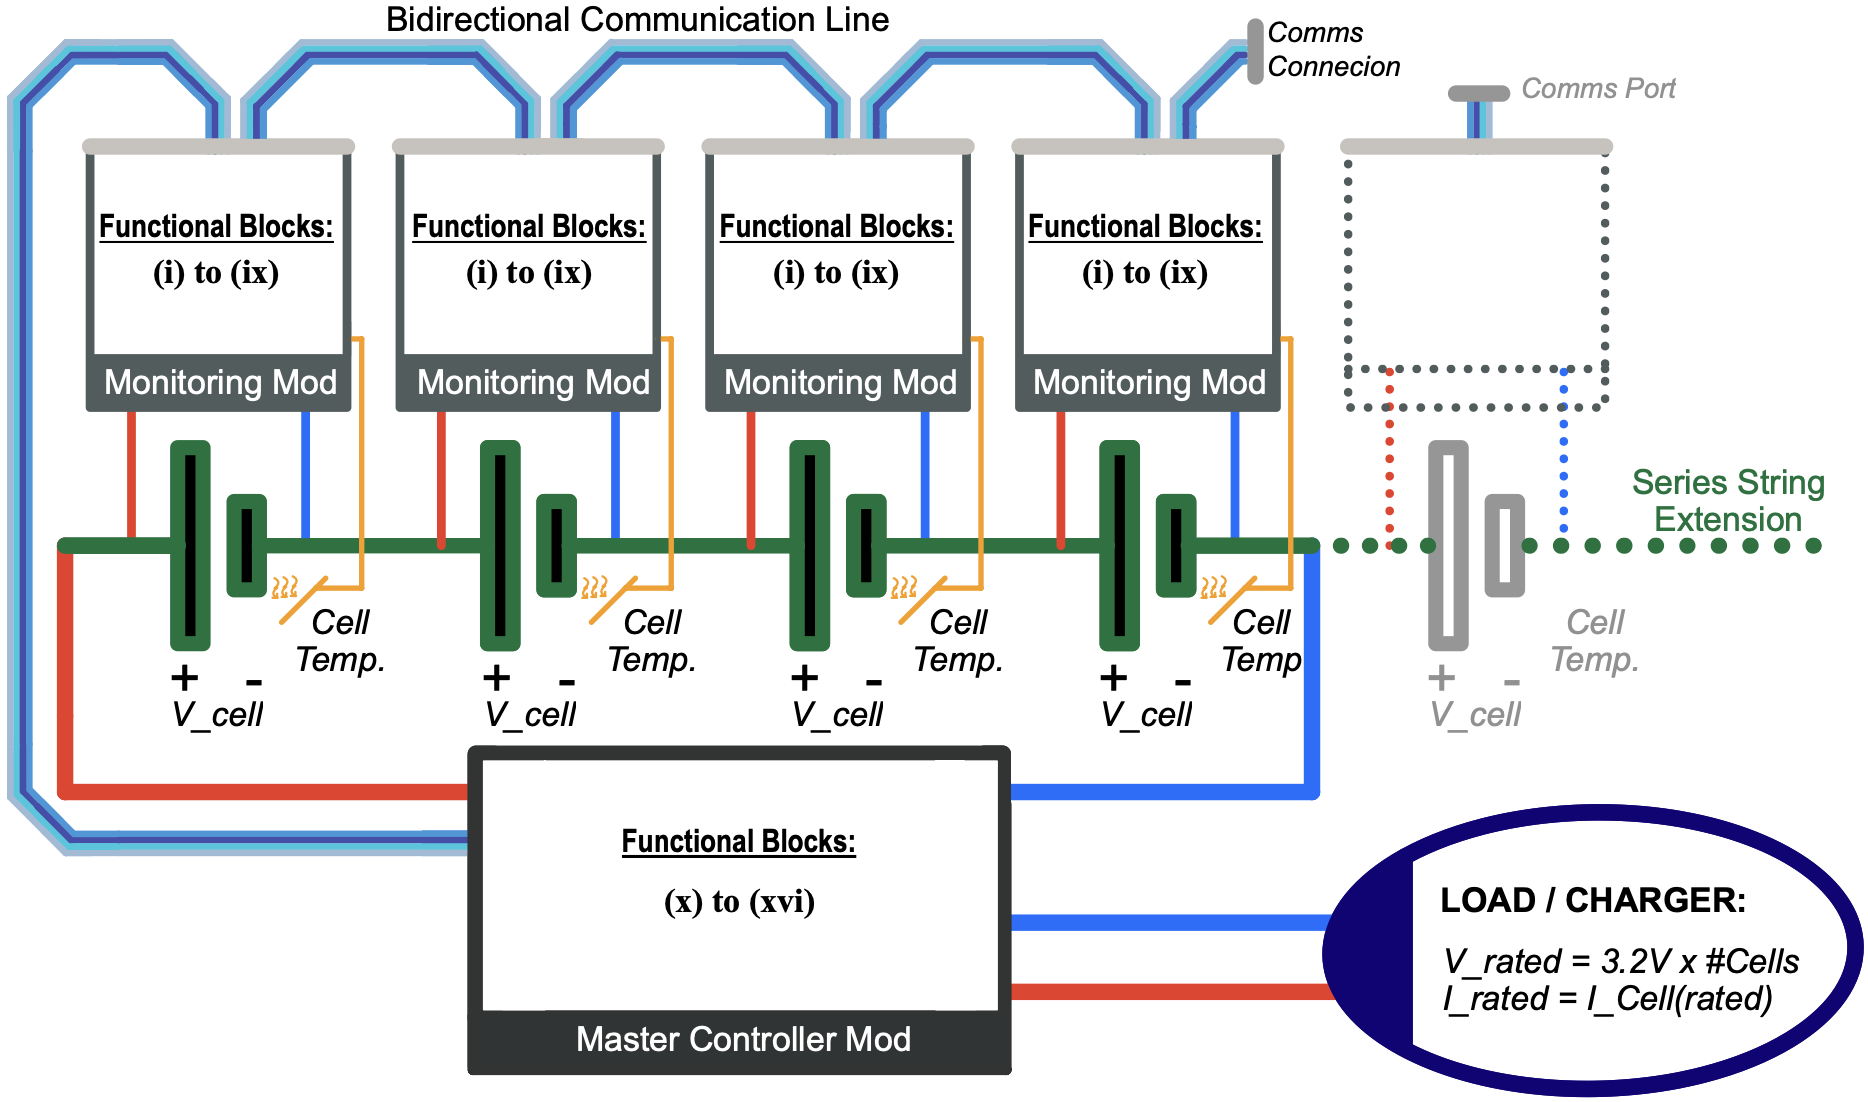
\includegraphics[width=0.7153\textwidth]{Skripsie_LaTeXTemplate/Figures/system_BLOCK_dia.png}
\caption{System Design Functional Blocks}
\label{fig:systOVV_Diagram}
\end{figure}
\noindent
The design of the BMS is organized into distinct functional blocks, each associated with specific subsystems. For a detailed breakdown of these blocks as depicted in figure \ref{fig:systOVV_Diagram}, refer to the subsequent table outlining the primary components of the design.
\begin{table}[h]
    \centering
    \caption{Functional Blocks and Subsystems}
    \label{tab:functional_subsystems}
    \begin{tabular}{|p{0.6cm}|p{6.cm}|p{8.4cm}|}
        \hline
        \textcolor{white}{.} & \textbf{Functional Block} & \textbf{Subsystems} \\
        \hline
        \hline
        \textcolor{white}{.} & \ref{subsec:moni_mods} \emph{Monitoring Module:} & \textcolor{white}{.} \\
        \hline
        \textbf{i} & \hyperref[subsubsec:MM_terminals_dsgn]{Cell Connection} & Parasite hookup \& Inline fuse protection \\
        \hline
        \textbf{ii} & \hyperref[subsubsec:PWR_supply_dsgn]{Voltage Regulation} & 5V Boost power supply \\
        \hline
        \textbf{iii} & \hyperref[subsubsec:force_RESET]{Supply Jumper \& Force Reset} & Programmmer mode \& Mosfet hard reset \\
        \hline
        \textbf{iv} & \hyperref[subsubsec:MM_MC]{Monitoring Microcontroller} & DFR(ATmega32U4) Arduino-Based System \\
        \hline
        \textbf{v} & \hyperref[subsubsec:IntTemp_and_DB_LED]{Onboard Diagnostics} & Internal temperture sensor \& Debug LEDs \\
        \hline
        \textbf{vi} & \hyperref[subsubsec:adc_design]{Cell Voltage Measurement} & Analog to digital converter \& precision reference \\
        \hline
        \textbf{vii} & \hyperref[subsubsec:DL_Designn]{Cell Balancing} & Mosfet passive dump load  \\
        \hline
        \textbf{viii} & \hyperref[subsubsec:ExtTemp_]{Cell Temperature Measurement} & External sensor for ambient temperature \\
        \hline
        \textbf{ix} & \hyperref[subsubsec:iso_COMS]{Isolated Module Communication} & UART isolation \& transceiver logic \\
        \hline
        \textcolor{white}{.} & \ref{subsec:mstr_contt} \emph{Master Controller:} & \textcolor{white}{.} \\
        \hline
        \textbf{x} & \hyperref[subsubsec:mstr_terminals_dsgn]{Terminals \& Fuse Protection} & Battery \& load/charger connection \\
        \hline
        \textbf{xi} & \hyperref[subsubsec:mstr_Supp]{Power Supply} & 5V Buck converter \\
        \hline
        \textbf{xii} & \hyperref[subsubsec:ESP32_dsgn]{Master Microcontroller} & ESP32 DevKitcV4 Arduino-Based System\\
        \hline
        \textbf{xiii} & \hyperref[subsubsec:cur_sen_design]{Battery Current Measurement} & Series connected sensor \\
        \hline
        \textbf{xiv} & \hyperref[subsubsec:LCD_Dsgn]{System Information Display} & LCD and I2C interface \\
        \hline
        \textbf{xv} & \hyperref[subsubsec:relay_Dsgn]{Load/Charge Disconnect} & Latching DC contactor \\
        \hline
        \textbf{xvi} & \hyperref[subsubsec:iso_COMS_Mstr]{Scalable Isolated Communication} & Broadcast UART isolation \\
        \hline
    \end{tabular}
\end{table}

\noindent
The development process of each element in Table \ref{tab:functional_subsystems} will be presented in the subsections: \ref{subsec:moni_mods} \& \ref{subsec:mstr_contt}. a Holistic and comprehensive design process was adopted, where the PCB design, circuit element design, and design calculations were performed simultaneously. This approach ensured a seamless integration between the circuitry and the PCB layout, resulting in an optimized hardware design. Each step of the design process involved meticulous attention to detail, considering factors such as component specifications, performance requirements, and manufacturability. Component selection played a pivotal role in achieving the desired functionality and reliability of the system. Extensive research was conducted, sifting through a vast array of datasheets to identify the most suitable components for each specific application.
%########################################################
\section{Monitoring Modules Design}\label{subsec:moni_mods}
%########################################################
\subsubsection{Design Outline}\label{subsec:mmmm1}
%########################################################
\begin{figure}[h!]
\centering
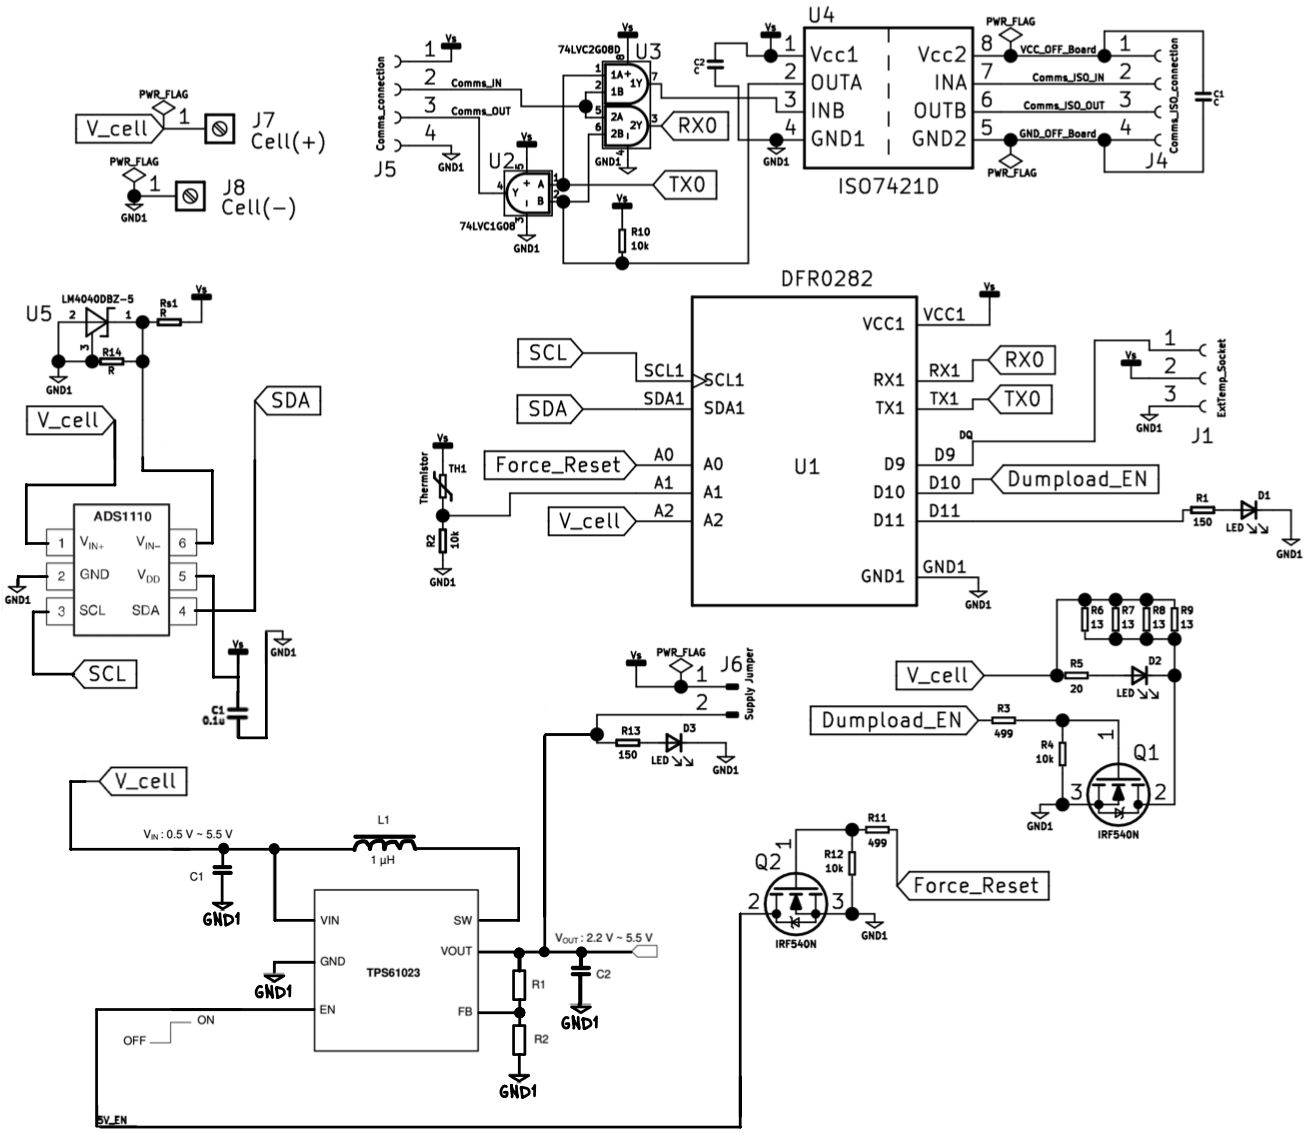
\includegraphics[width=0.9\textwidth]{Skripsie_LaTeXTemplate/Figures/Monitor_Schematic.png}
\caption{Monitoring Module Schematic Diagram}
\label{fig:Monitor_Schema}
\end{figure}

\noindent
Refer to Figure \ref{fig:Monitor_Schema} above for the comprehensive schematic of the monitoring system modules. As delineated in the system overview, the design comprises distinct subsystems working in tandem to form a precise measurement and control platform. A thorough examination of each subsystem's circuit design and component selection is presented in the subsequent section. The \hyperref[subsec:mmmm3]{PCB design} further demonstrates the system's adherence to the design requirements to fit on top of a prismatic LFP cell.
%########################################################
\subsubsection{Circuit Designs \& Component Selection}\label{subsec:mmmm2}
%########################################################
\textbf{\emph{Cell Connection}}\label{subsubsec:MM_terminals_dsgn}

\begin{figure}[h!]
\centering
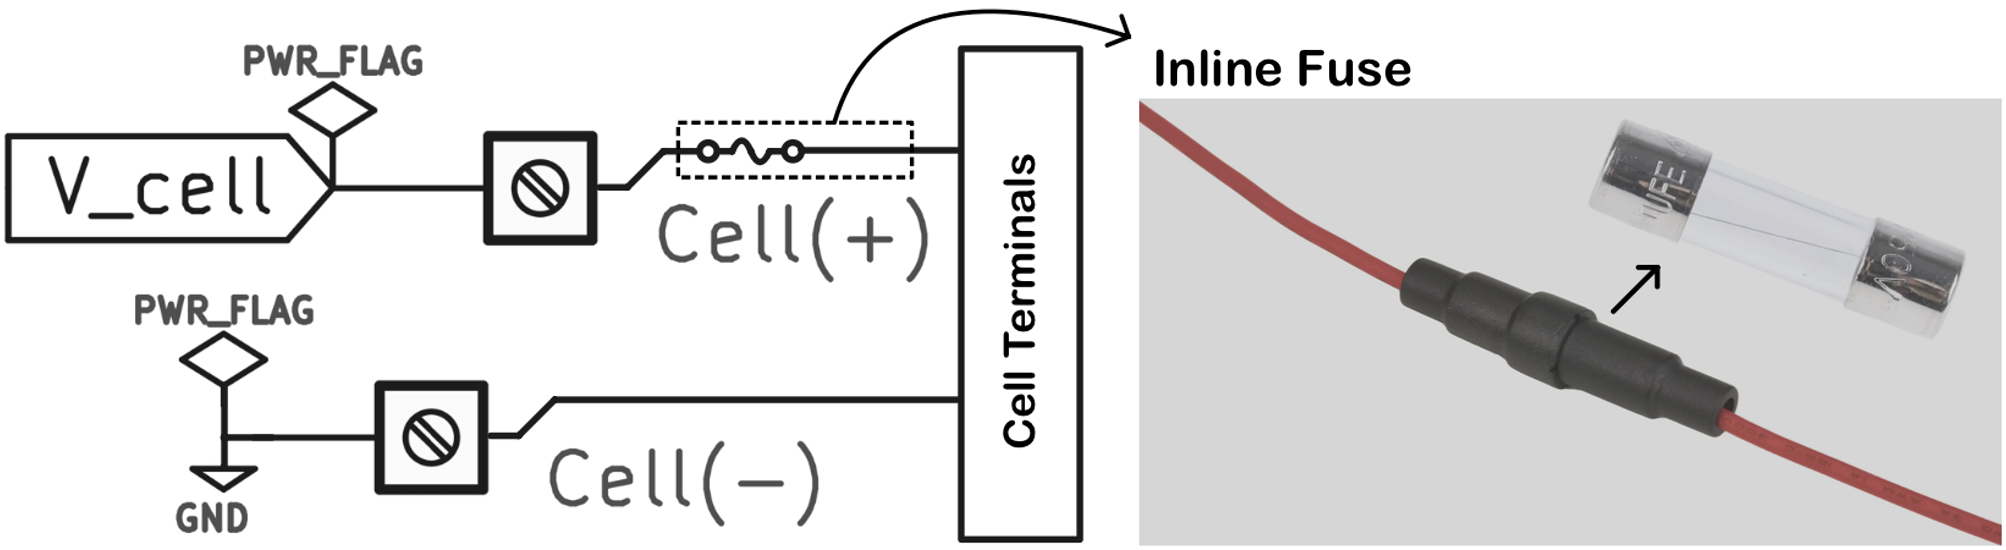
\includegraphics[width=0.4\textwidth]{Skripsie_LaTeXTemplate/Figures/MM_Terminals_Designn.png}
\caption{Monitoring Mod Terminals and Fuse Protection \cite{inlineFuse}}
\label{fig:MM_D9}
\end{figure}
\noindent
A two-pin through-hole PCB connector facilitates cell connection, employing a METZ Connect terminal block rated at 15A to ensure reliable connection beyond peak current demands. The monitoring boards, connecting in parallel to each cell within a series, enable module data acquisition and power draw from the data line, negating external power supply needs. Over-current protection is implemented with a 5mm x 20mm glass fuse, rated at 1.5A, linking the cell's positive terminal to the module, allowing safe 1A discharge by the balancing load during monitoring. While resettable fuses could improve future designs, they are not essential for the current prototype.\newline\newline
%########################################################
\noindent
\textbf{\emph{Voltage Regulation}}\label{subsubsec:PWR_supply_dsgn}\newline
\noindent
To ensure the high precision monitoring system functions optimally, it is crucial to guarantee a stable and accurate power supply to the board. While the system’s microcontroller can operate with voltage as low as 3V, it can’t reach its full functionality. Hence, the voltage level of the 3.2V LFP cell is insufficient to power the board correctly. The voltage is also fluctuating when the cell is being discharged and the ADC used to measure the cell voltage needs a high precision fixed reference voltage to obtain accurate measurements. For a solution we require a voltage step up to 5V, this will also provide a higher logic level for better resolution in the measurements.  

\begin{figure}[h!]
\centering
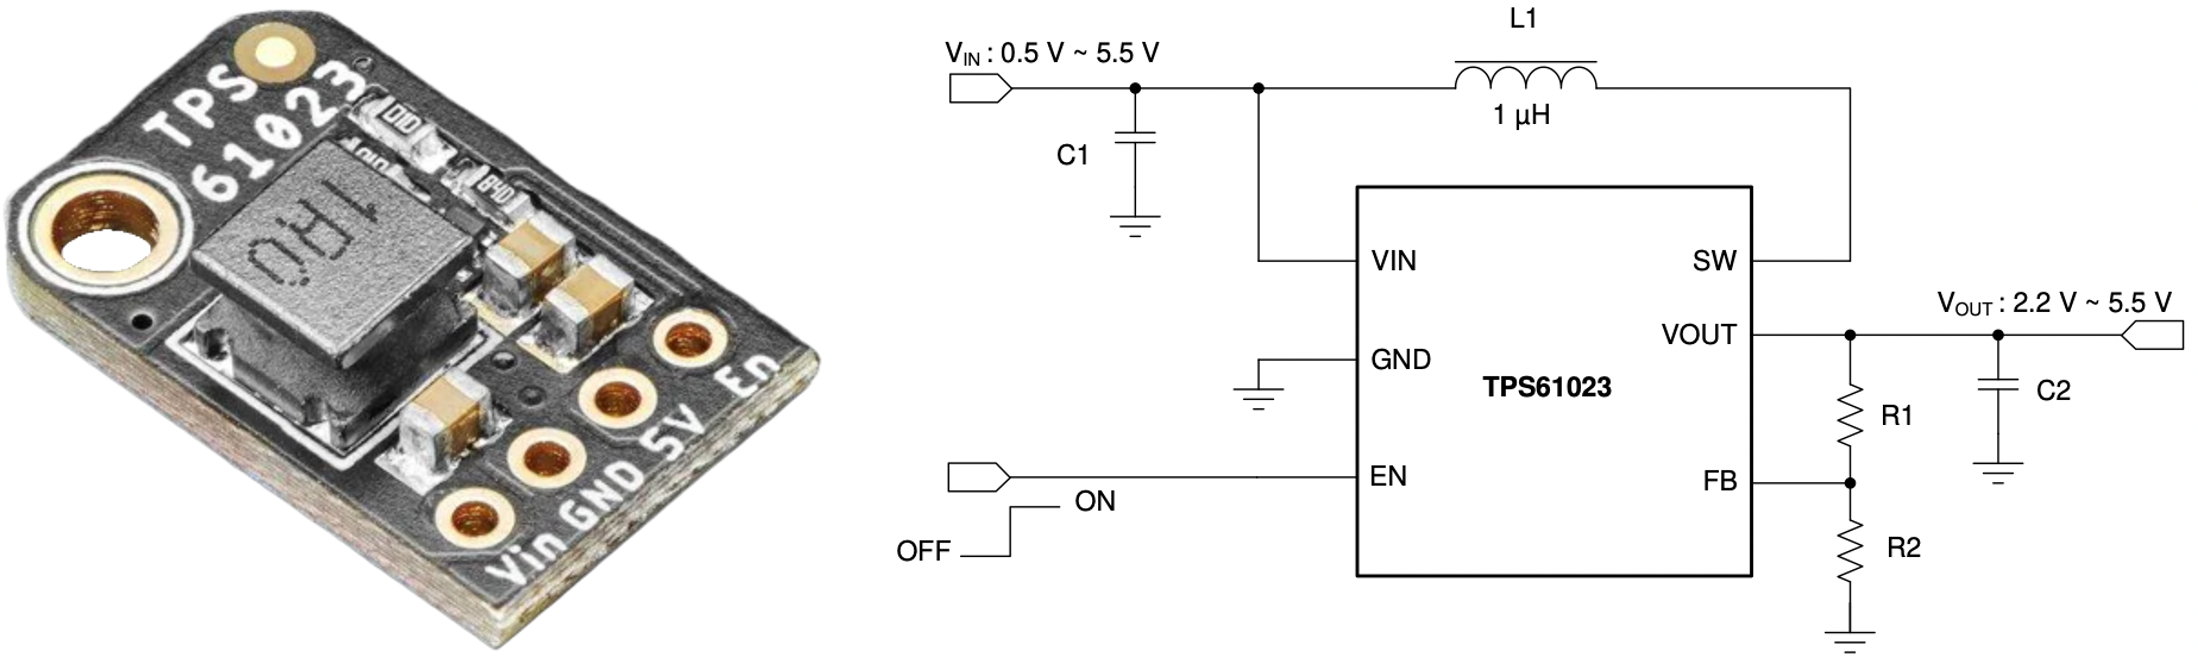
\includegraphics[width=0.6\textwidth]{Skripsie_LaTeXTemplate/Figures/PwrSupp_Designn.png}
\caption{MiniBoost 5V \cite{5vSupply}}
\label{fig:MM_D8}
\end{figure}
\noindent
a Mini-booster utilizing a charge-pump topology with the TPS61023 chip from Texas Instruments is used to preform the voltage regulation. The booster can supply up to 1A current at 5V with a 1\% precision making it the optimal design chose for this purpose.\newline\newline
%########################################################
\noindent
\textbf{\emph{Supply Jumper \& Force Reset}}\label{subsubsec:force_RESET}\newline
\noindent
A power supply jumper is integrated in the battery cell-based system to safely disconnect it from the power source during microcontroller programming, as depicted in figure \ref{fig:MM_D7}. This jumper serves a dual purpose: it establishes a "programmer mode" for safe microcontroller programming and enables reconnection to the power source post-programming, ensuring operational flexibility and system protection during firmware updates.

\begin{figure}[h!]
\centering
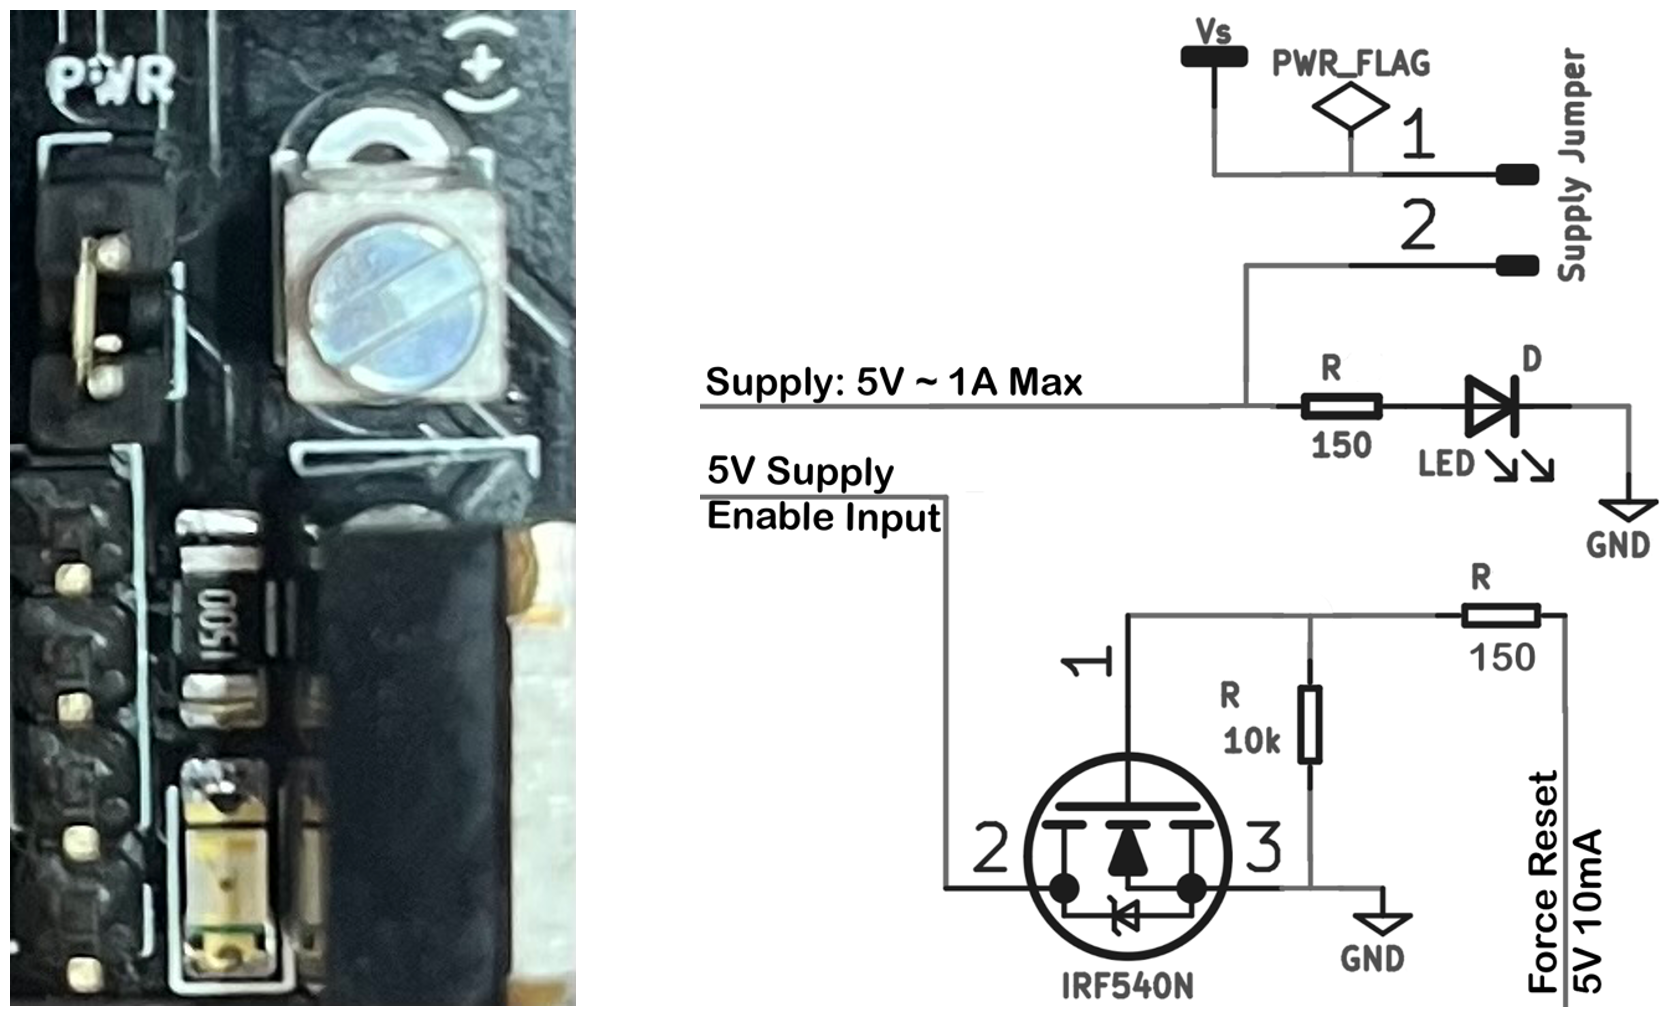
\includegraphics[width=0.38\textwidth]{Skripsie_LaTeXTemplate/Figures/ProgJmp_FReset_Designn.png}
\caption{Power Supply Connection \& Force Reset}
\label{fig:MM_D7}
\end{figure}

\noindent
An emergency reset circuit is included, utilizing a mosfet as a low-side switch to momentarily ground the enable pin of the TPS61023 chip, thereby initiating a system restart. This force reset functionality is vital for addressing unforeseen microcontroller errors, glitches, or transient faults, enabling a quick system return to a known, stable state without manual intervention.\newline\newline
%########################################################
\noindent
\textbf{\emph{Monitoring Microcontroller}}\label{subsubsec:MM_MC}\newline
\noindent
The DFR0282 microcontroller, chosen for its compact size fitting aptly between cell terminals, facilitates on-the-fly programming alterations via its micro-USB feature. Its compatibility with Arduino Leonardo simplifies rapid code modifications in the Arduino environment, meeting the project's technical requisites efficiently.

\begin{figure}[h!]
\centering
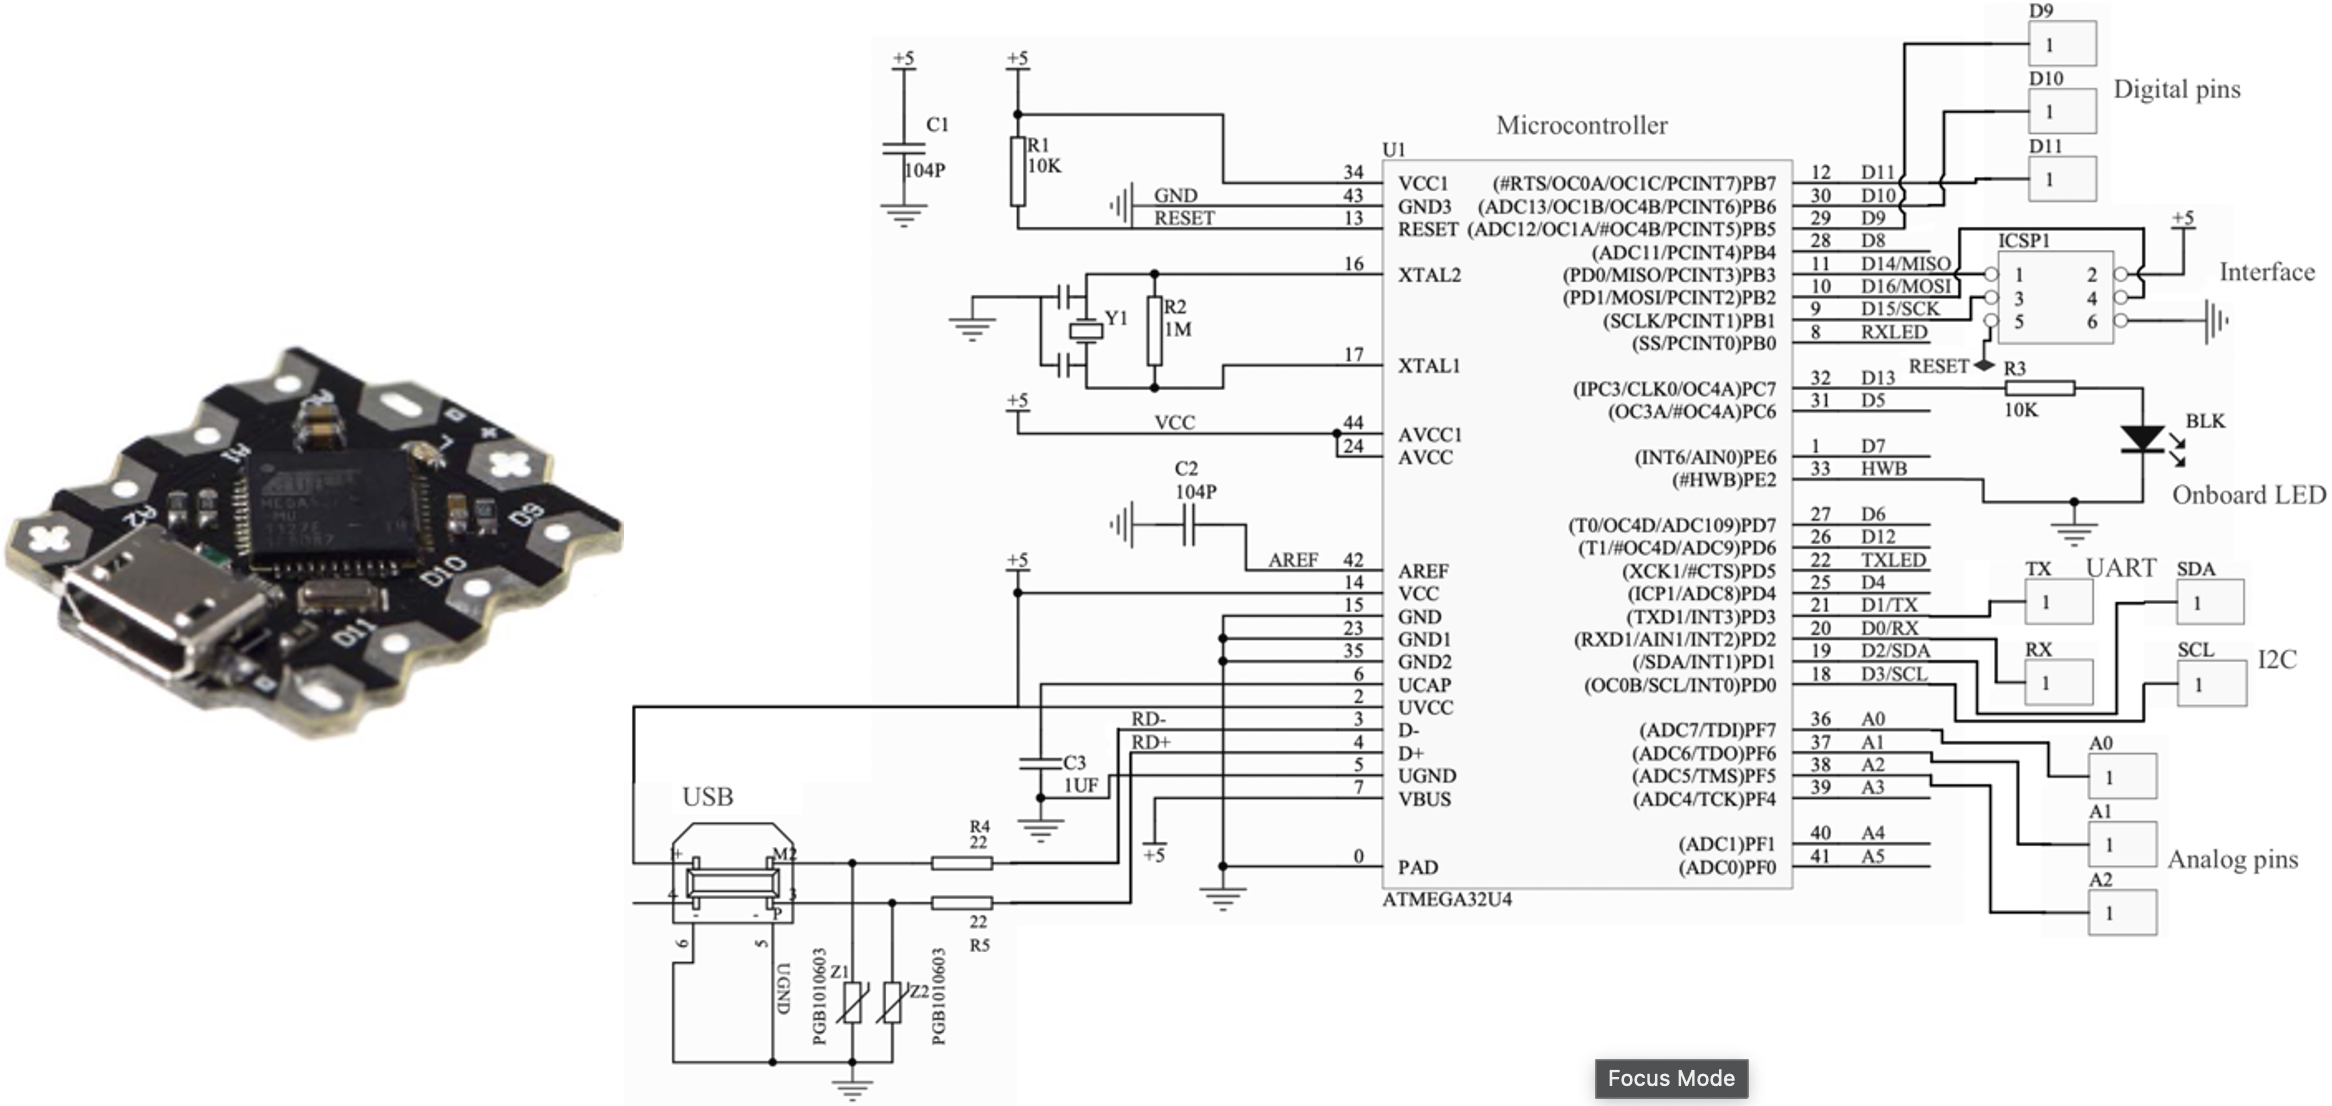
\includegraphics[width=0.7\textwidth]{Skripsie_LaTeXTemplate/Figures/MM_MircoCont_Designn.png}
\caption{DFR0282 - (ATmega32U4) Microcontroller \cite{beetle}}
\label{fig:MM_D6}
\end{figure}

\noindent
Equipped with the ATmega32U4 chip and accompanying conditioning circuitry, the DFR0282 module provides six General Purpose Input/Output (GPIO) pins, I2C, and UART pins. This pin configuration aligns with system requirements, ensuring full utilization of available pins for designated functions as detailed in the subsequent table, thereby enhancing the system's functional efficacy.

\begin{table}[h]
    \centering
    \caption{Monitoring Microcontroller Pin Out}
    \label{tab:Beetle_PinOut}
    \begin{tabular}{|c|c|c|}
        \hline
        \textbf{DFR0282-Pin} & \textbf{Configuration} & \textbf{Utility} \\
        \hline
        \hline
        0 & RX & Serial communication receive channel \\
        \hline
        1 & TX & Serial communication transmit channel \\
        \hline
        2 & SDA & I2C data channel for external ADC \\
        \hline
        3 & SCL & Clock channel for I2C sampling \\
        \hline
        9 & Digital GPIO & External temperature sensor digital input \\
        \hline
        10 & Digital GPIO & Cell balancing dump-load enable pin \\
        \hline
        11 & PWM Channel & LED for system debug messages \\
        \hline
        A0 & Digital GPIO & Force reset enable pin \\
        \hline
        A1 & Analog Channel & Internal temperature sensor analog input \\
        \hline
        A2 & Analog Channel & Cell voltage analog input \\
        \hline
    \end{tabular}
\end{table}

%########################################################
\noindent
\textbf{\emph{Onboard Diagnostics}}\label{subsubsec:IntTemp_and_DB_LED}

\begin{figure}[h!]
\centering
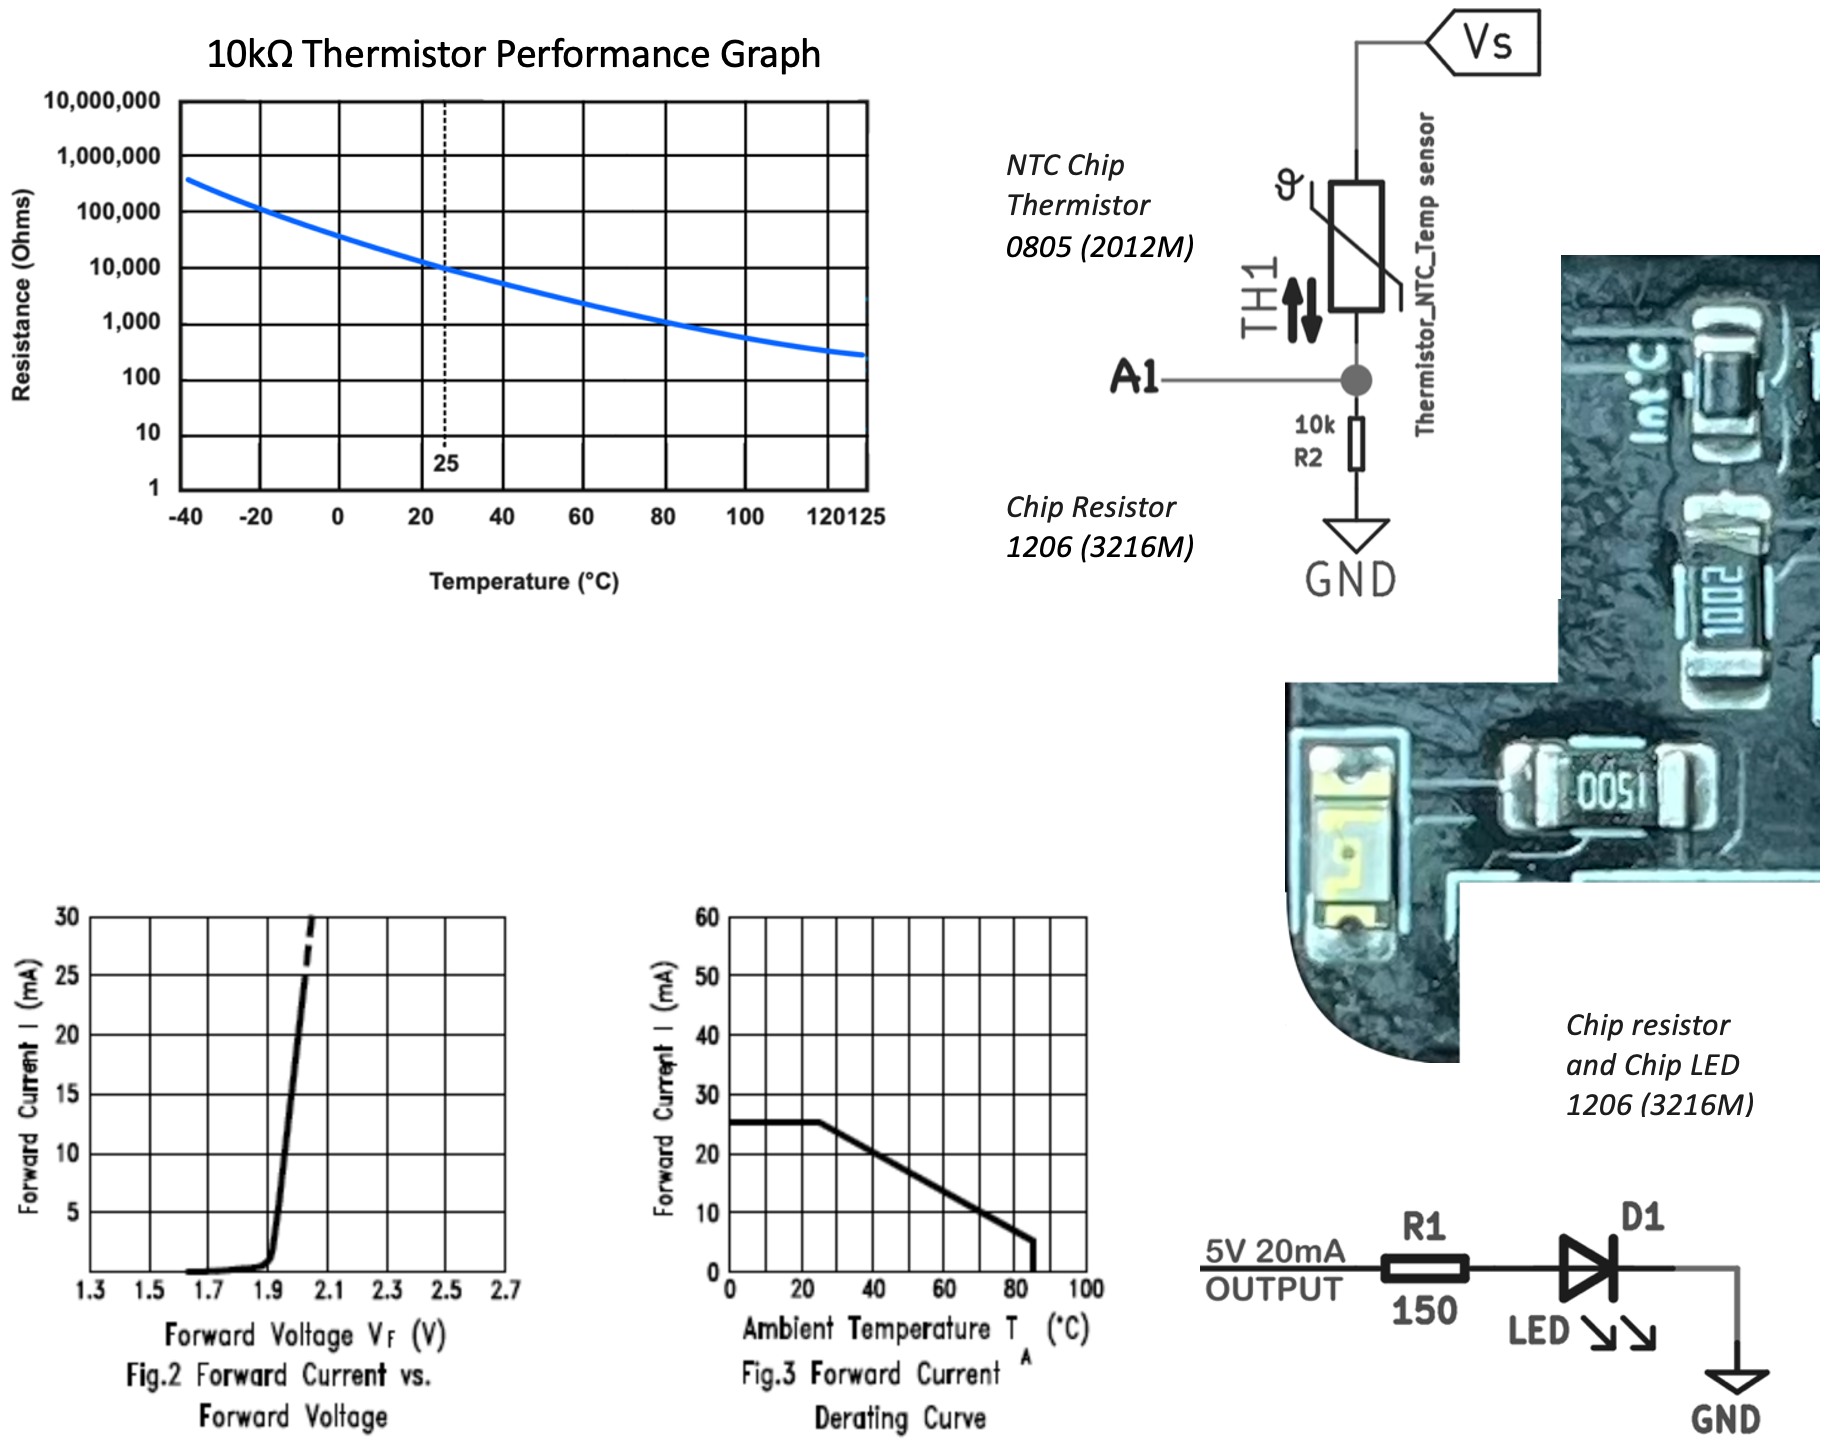
\includegraphics[width=0.5\textwidth]{Skripsie_LaTeXTemplate/Figures/IntTemp_LED_Designn.png}
\caption{NTC Temperature Sensor \cite{IntTemp} \& Debug LED \cite{LED}}
\label{fig:MM_D5}
\end{figure}
\noindent
\emph{Internal Temperature Measurement:}\newline
\noindent
An on-board temperature sensor is crucial for real-time thermal management, ensuring operational safety and optimizing performance. The circuit employs a TE Connectivity Thermistor in a voltage divider configuration with a fixed \(10k\Omega\) resistor. The thermistor's resistance (\( R_{th} \)) varies with temperature (graph presented in figure \ref{fig:MM_D5}), affecting the voltage (\( V_{out} \)) at the microcontroller's analogue input pin as per the following equations.
\[ R_{th} = R_0 \cdot \exp \left( \frac{\beta}{T} - \frac{\beta}{T_0} \right) \hspace{0.5cm} \& \hspace{0.5cm} V_{out} = 5V \cdot \left( \frac{R_{th}}{R + R_{th}} \right) \]
\noindent
\emph{System Debug LED:}\newline
\noindent
An LED indicator is instrumental for providing immediate, visible feedback regarding system debug messages, aiding in swift diagnosis and rectification of operational issues.
\[ R_{limiting} = \frac{V_s - V_f}{I} = \frac{5V - 2V}{0.02A} = 150 \Omega \]
%########################################################
\noindent
\textbf{\emph{Cell Voltage Measurement}}\label{subsubsec:adc_design}

\begin{figure}[h!]
\centering
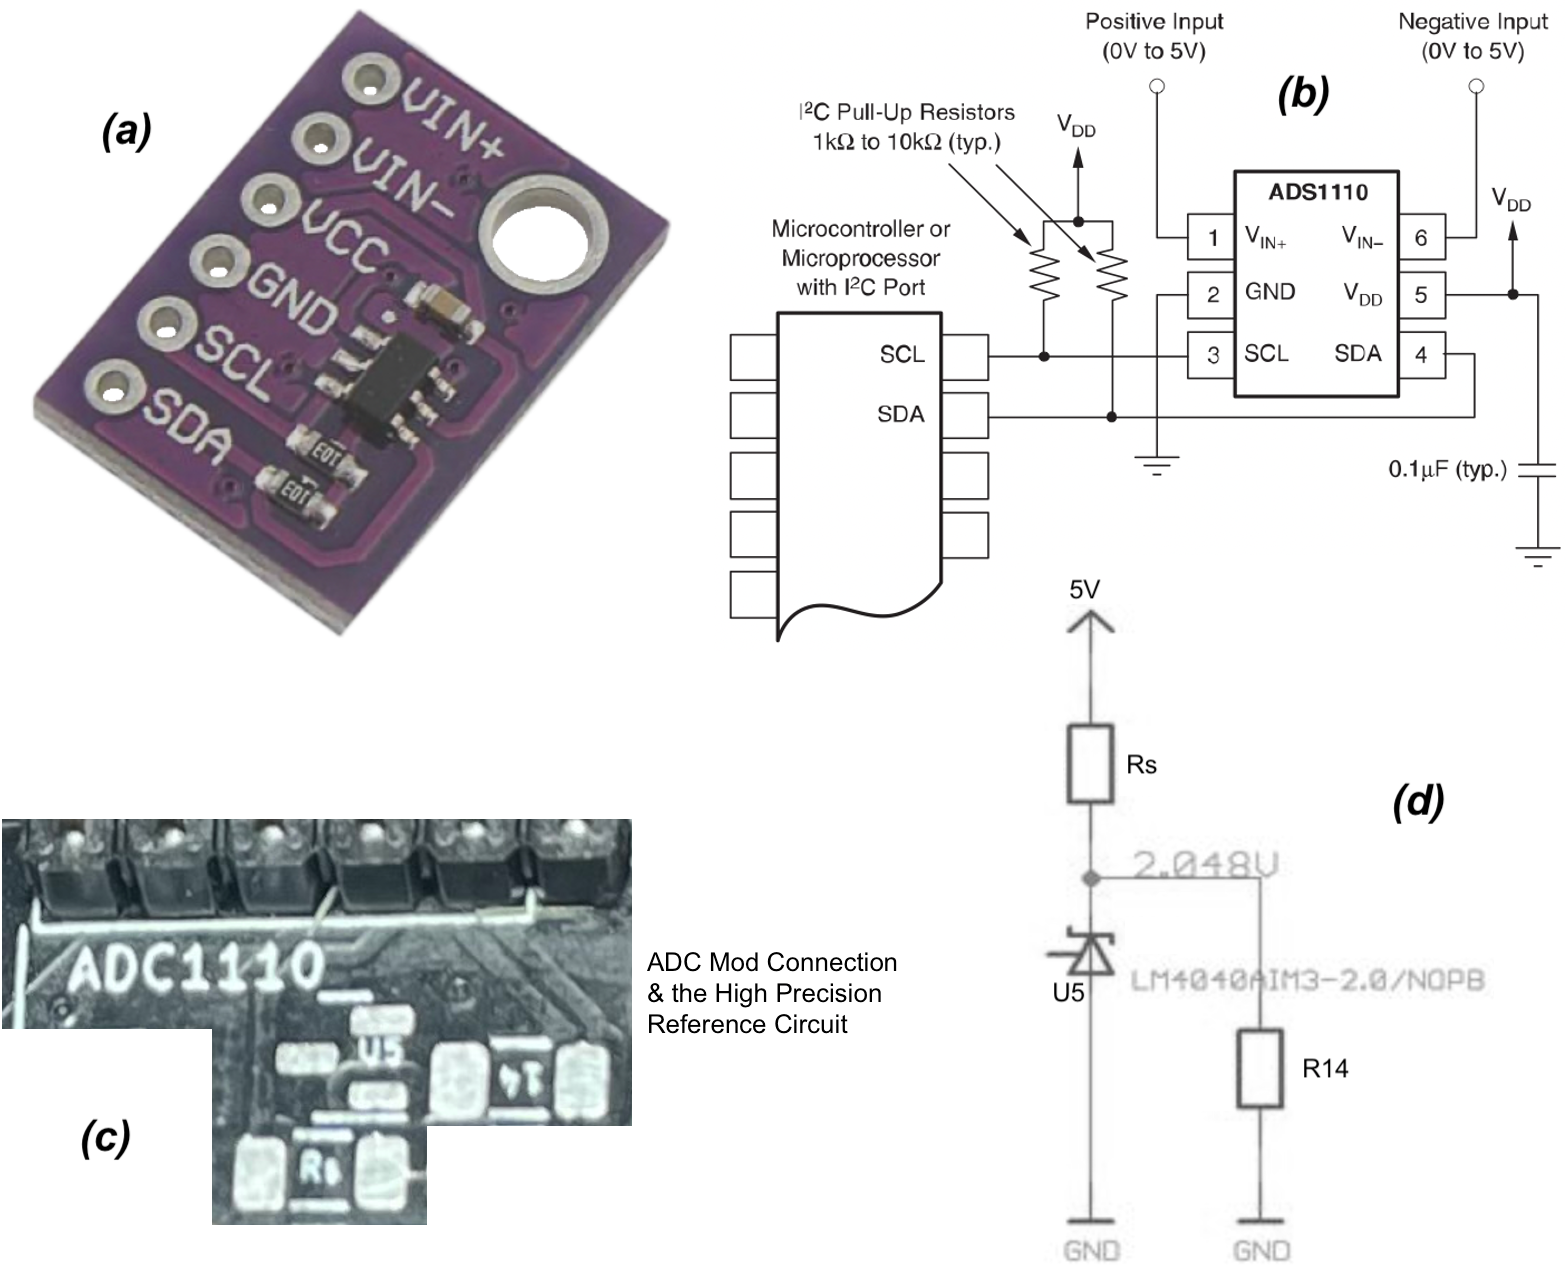
\includegraphics[width=0.5\textwidth]{Skripsie_LaTeXTemplate/Figures/ADC_Designn.png}
\caption{(a)16bit ADC (b)ADS1110 Design\cite{TheADC} (c)2.048V Ref. (d)LM4040 Design\cite{PrecRef}}
\label{fig:MM_D1}
\end{figure}
\noindent
Accurate cell voltage measurement is crucial for cell monitoring. While the DFR0282 microcontroller has an onboard 8-bit ADC for backup measurement, a high-precision measurement is achieved using an external 16-bit ADC, the ADS1110. As depicted in figure \ref{fig:MM_D1}\textbf{(a)}, the ADS1110 interfaces with the microcontroller via 2K2 pull-up resistors on its I2C lines, operating at a baud rate of 9600. Powered by the microcontroller's 5V and ground lines, the ADS1110, with a sample rate of 240 SPS, offers a resolution of approximately 0.00003125V, as calculated by the formula below.
\[
\text{Resolution} = \frac{V_{\text{ref}}}{2^{\text{N}}} = \frac{2.048V}{2^{\text{16 bits}}} = 31.25 \mu
\]
\noindent
A stable external 2.048V reference is essential for maintaining the ADC's precision, as depicted in figure \ref{fig:MM_D1}\textbf{(c)}. The circuit, as shown in figure \ref{fig:MM_D1}\textbf{(d)}, utilizes the LM4040AIM3-2.0/NOPB shunt voltage reference chip, a \(750 \, \Omega\) series resistor (\(R_s\)), and a \(10 \, k\Omega\) shunt resistor (\(R_{sh}\)). The anode and NC pin of the LM4040AIM3-2.0/NOPB are grounded, while the cathode pin connects to a junction, also connected to \(R_s\) and \(R_{sh}\).
\[
I_{ref} = \frac{V_{supply} - V_{ref}}{R_s} = \frac{5V - 2.048V}{750 \, \Omega}
\]
\noindent
The formula above determines the current through the LM4040AIM3-2.0/NOPB chip (\(I_{ref}\)), and the total current through \(R_s\) is given by the following equation.
\[
I_{R_s} = I_{ref} + I_{sh} = I_{ref} + \frac{V_{ref}}{R_{sh}}
\]
\noindent
This design ensures a stable reference voltage across various operating conditions, thus preserving the accuracy of the 16-bit ADC for precise cell voltage measurement.\newline\newline
%########################################################
\noindent
\textbf{\emph{Cell Balancing}}\label{subsubsec:DL_Designn}\newline
\noindent
Cell balancing is crucial for managing LFP battery packs where series-connected cells exhibit variations in capacity, internal resistance, and charge characteristics, leading to voltage imbalances that affect battery life and safety. It aims to equalize the SOC across cells. Two prevalent techniques exist: active and passive balancing. Active balancing employs switches and capacitors for charge transfer, presenting efficiency albeit at higher complexity and cost. Conversely, passive balancing dissipates excess charge through resistors, offering simplicity, cost-effectiveness, and reliability, often making it a preferred choice in robust system designs over the marginal efficiency benefits of active balancing.

\begin{figure}[h!]
\centering
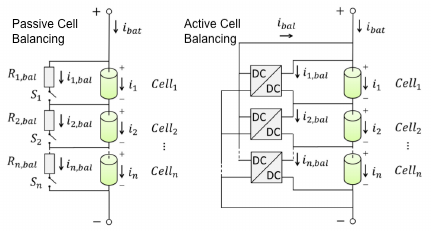
\includegraphics[width=0.4\textwidth]{Skripsie_LaTeXTemplate/Figures/actVSpass.png}
\caption{Activate vs Passive Balancing \cite{generic}}
\label{fig:actVSpass}
\end{figure}
\noindent
A passive balancing circuit was chosen for the cell modules, with balancing current as a pivotal factor. To ascertain the dump load size for each cell in a 105Ah 3.2V LFP series-connected battery pack, it's necessary to consider both the maximum charging current and the required balancing current for effective balancing. The EVE Energy cell datasheet \cite{eve} recommends a maximum charging current of 1C (105A) for the battery pack, thus a balancing current of about 1\% of the maximum charging current, or approximately 1A, is deemed suitable for the dump load design per cell.

\begin{figure}[h!]
\centering
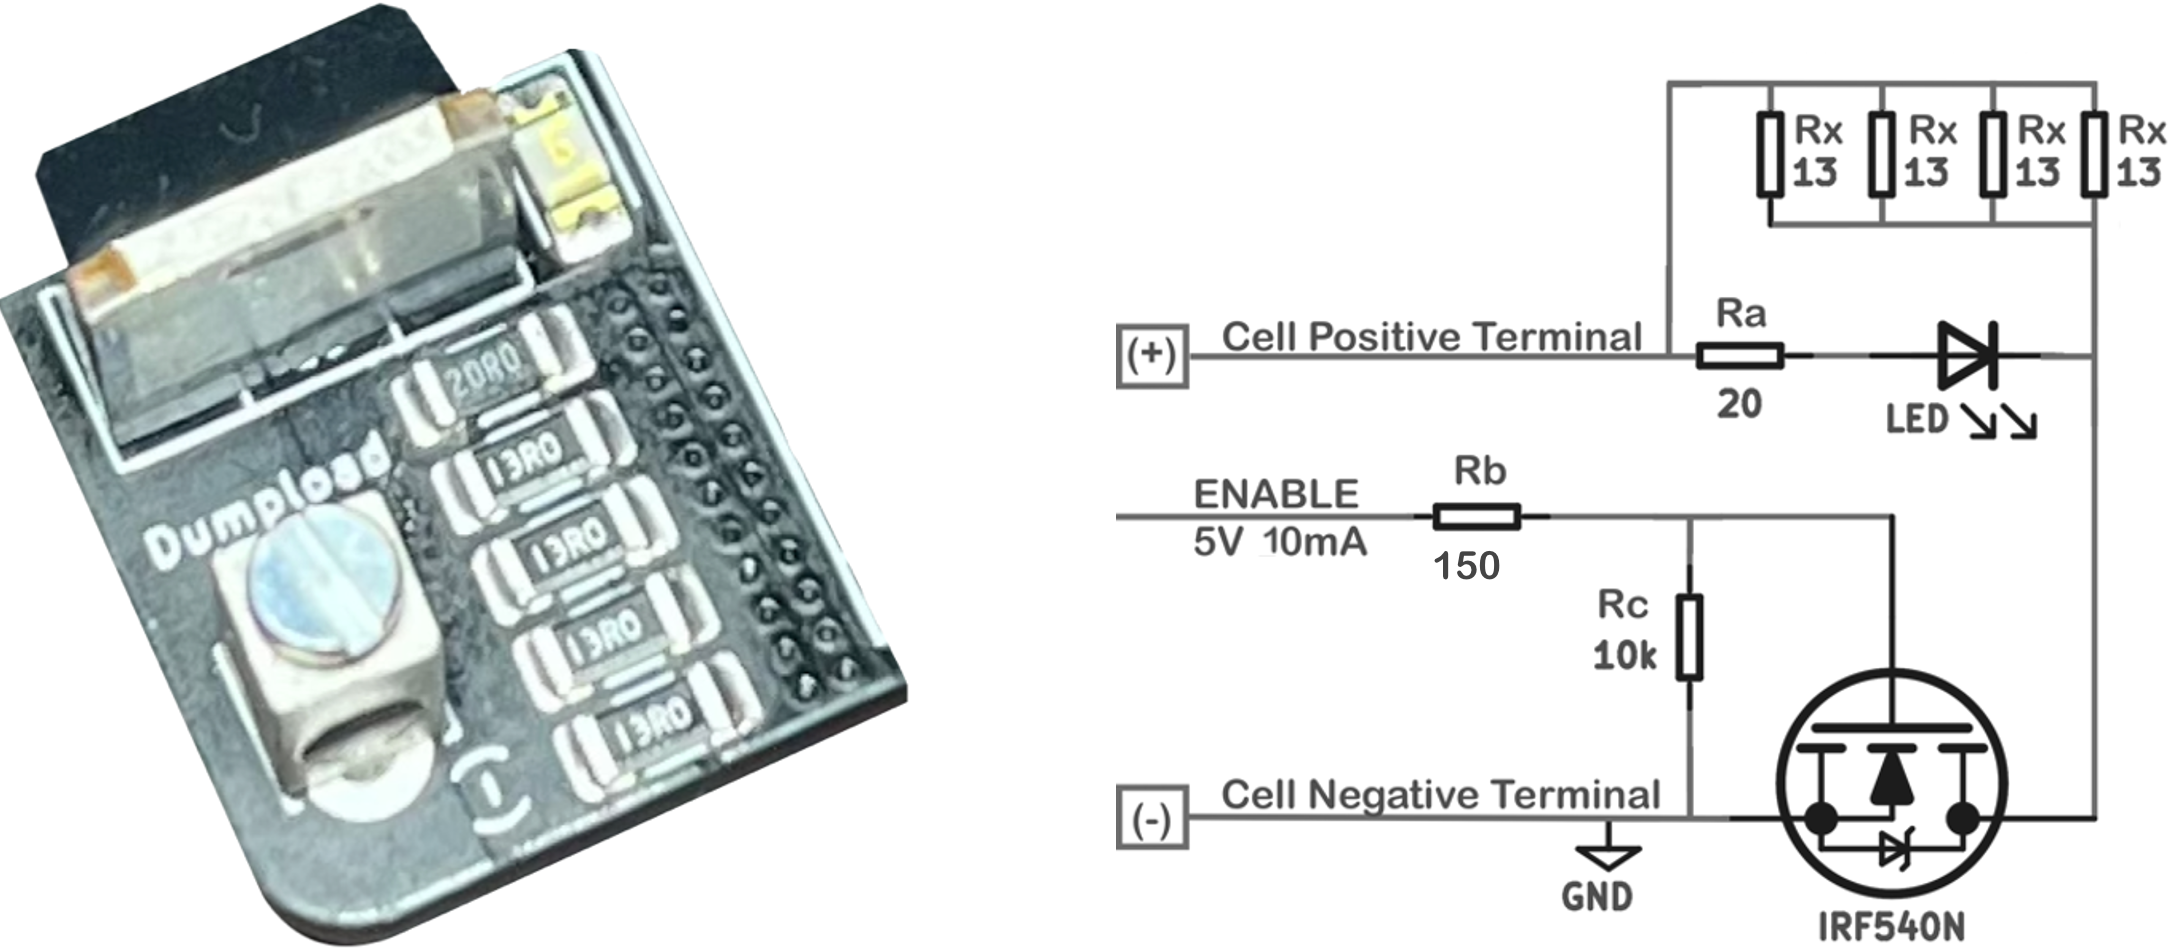
\includegraphics[width=0.5\textwidth]{Skripsie_LaTeXTemplate/Figures/DmpLoad_Designn.png}
\caption{Balancing Dump-load Design}
\label{fig:MM_D3}
\end{figure}
\noindent
The load is made up of four $13\Omega$ chip resistors in parallel.
\begin{equation}
R_{\text{Dump-Load}} = (\frac{1}{13\Omega} \cdot 4)^{-1} = 3.25\Omega
\end{equation}
This resistance value results in a balancing current just below 1A.
\begin{equation}
I_{\text{Balancing}} = \frac{3.2V}{3.25\Omega} = 0.985A
\end{equation}
To ensure that the resistors are thermally capable of handeling the balancing current we need to look at their power rating.
\begin{equation}
P_{\text{Dump-Load}}(Min.) = (0.985A)^{2} \cdot 3.25\Omega = 3.153W
\end{equation}
Since the resistors are connected in parallel the power rating for the dumpload is given by the equation below.
\begin{equation}
P_{\text{Dump-Load}} = P_{13\Omega-Resistor} \cdot 4
\end{equation}
\noindent
Therefor a high power thin film $13\Omega$ chip resistor from SUSUMU \cite{CHIPrr}, with a power rating of $1W$ was chosen for safe operation of the load.\newline\newline
\noindent
\emph{Low-side Switch:}\label{subsubsec:LS_SW}\newline
\noindent
The dump-load is controlled by a microcontroller with a desire output of 20mA on its gpio pins. a High signal of 5V on the pin is used to switch a Power Mosfet. The mosfet is used in a low-side switch configuration and has a gate threshold voltage of 2V. The following calculation was done to select the appropriate gate current limiting resistor \cite{mos}.
\begin{equation}
R = \frac{\Delta V}{I_{Gate}} = \frac{5V - 2V}{20mA} = 150\Omega
\end{equation}
\noindent
A $10k\Omega$ resistor is typically used as a pull-down resistor in a 5V system due to its balance of limiting current, reducing power consumption, and ensuring reliable logic level interpretation.\newline\newline
%########################################################
\noindent
\textbf{\emph{Cell Temperature Measurement}}\label{subsubsec:ExtTemp_}\newline
\noindent
Designed to be positioned at the cell's negative terminal (current entry \& exit point), the external temperature sensor, DS18B20, facilitates effective cell thermal monitoring crucial for detecting temperature alterations under heavy loads or charging, thereby enhancing battery safety and efficiency.

\begin{figure}[h!]
\centering
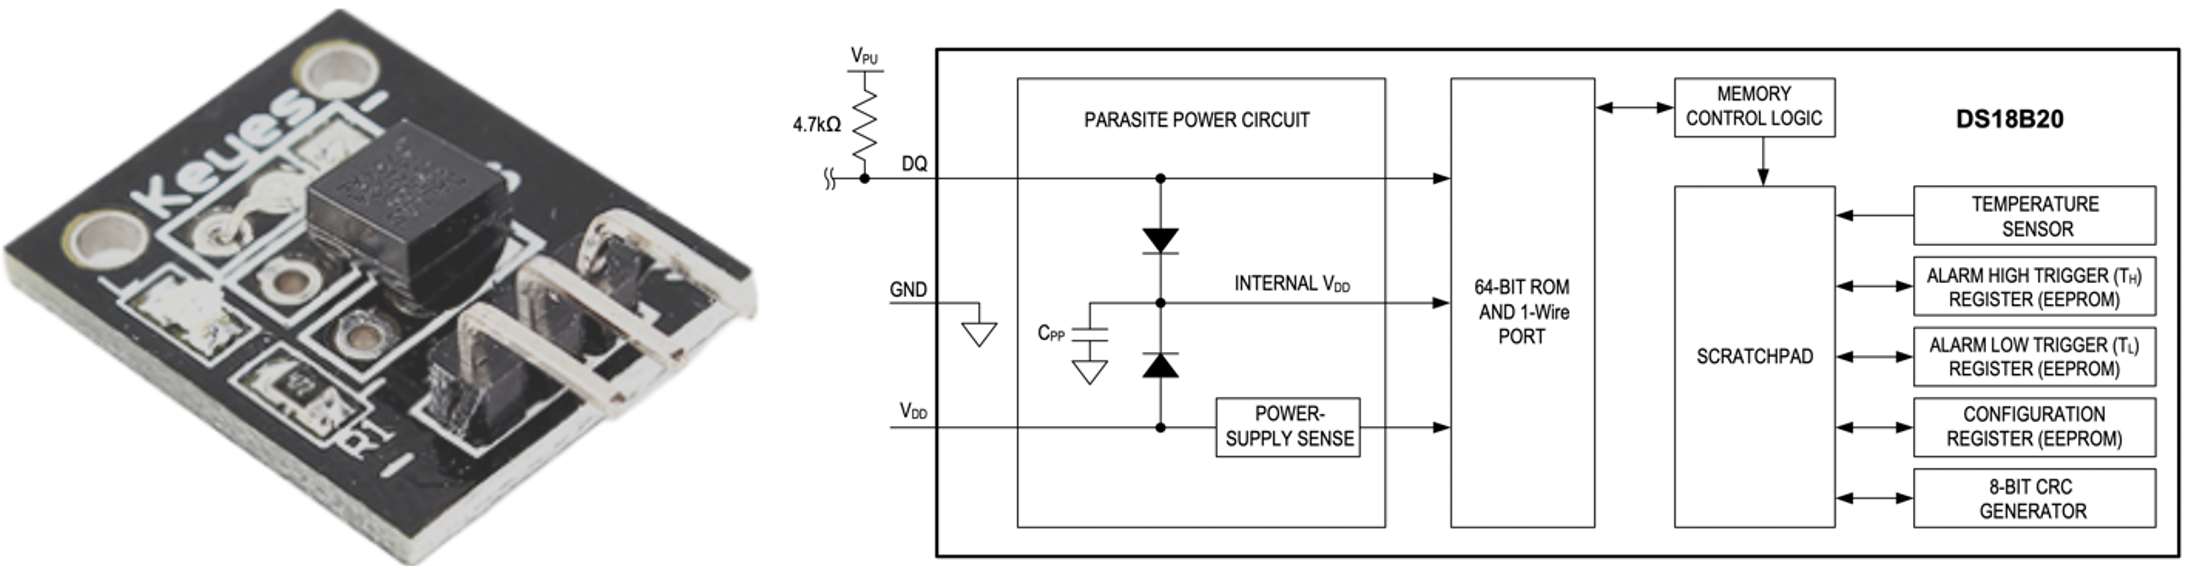
\includegraphics[width=0.65\textwidth]{Skripsie_LaTeXTemplate/Figures/ExtTemp_Designn.png}
\caption{External Temperature Sensor \cite{TheExtTempSen}}
\label{fig:MM_D4}
\end{figure}
\noindent
The DS18B20 ensures ±0.5°C accuracy within a -20°C to +85°C range, extendable to -55°C to +125°C. Operating at 5V with a 9 to 12-bit resolution range and "parasite power" capability, the DS18B20 eliminates the need for external power, making it a proficient choice for ambient cell temperature monitoring.\newline\newline
%########################################################
\noindent
\textbf{\emph{Isolated Module Communication}}\label{subsubsec:iso_COMS}\newline
\noindent
As delineated in the background study's section \ref{sec:commsMeth}, a comprehensive analysis guided the design choice of the ISO7421D (low-power dual-channel digital isolator chip) from Texas Instruments \cite{isooooCHIP} to isolate UART communication lines. Unlike optocouplers that requires external components for operation, the ISO7421D solely requires two bypass capacitors for supply decoupling. The devised architecture diverges from conventional series-connected isolated daisy-chain or parallel-connected isolated bus lines. Instead, ISO7421D chips are serialized, creating a communication line segmented by isolated barriers, each with two channels: one facilitating data transmission down the stack, and the other, upwards.\newline\newline
\noindent
This arrangement creates a bidirectional communication bus, wherein between each isolating barrier, signals are either tapped off using a receiver or tapped into the communication line via a transmitter, adhering to an asynchronous serial system protocol. Consequently, all modules along the communication line attain broadcast channel read and write access throughout the system. This configuration mitigates the limitations of common all-call and daisy-chain setups, which encounter scalability constraints due to the elevated output impedance on serial communication, attributed to parallel-arranged digital isolator chips. Such impedance escalation prompts the integration of output drivers to ensure proficient message transmission across the communication line. The novel communication system is illustrated in figure \ref{fig:MM_D2} below.

\begin{figure}[h!]
\centering
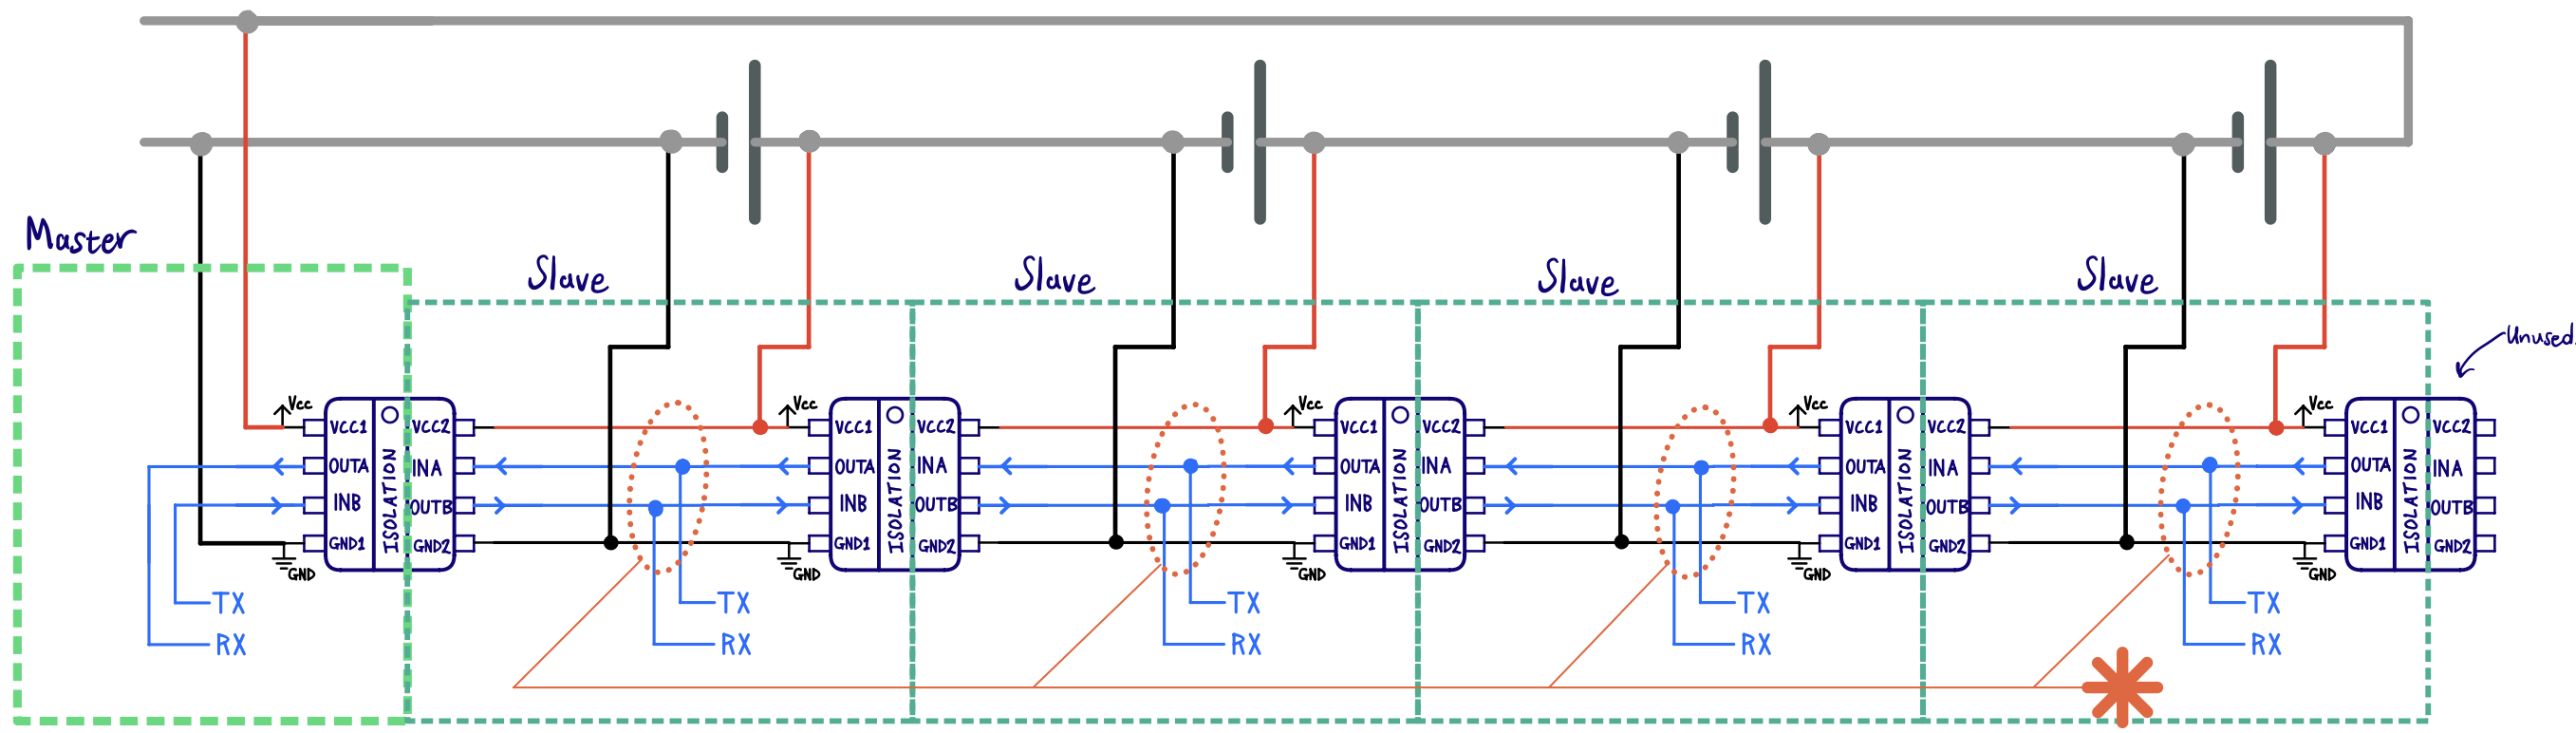
\includegraphics[width=1.0\textwidth]{Skripsie_LaTeXTemplate/Figures/COMMS_SELECT.png}
\caption{Isolated Communication Configuration}
\label{fig:MM_D2}
\end{figure}
\noindent
The design configuration above may incur bus contention (\textcolor{orange}{\textbf{*}}) during simultaneous data transmission by multiple transceivers, resulting in signal interference and data corruption. Addressing this issue involves the utilization of an asynchronous software protocol with sequential program timers, which allocates specific time slots for each transceiver to transmit data, thus eliminating overlap and resolving bus contention. To fortify against unforeseen simultaneous data transmission potentially harmful to the system, a communication bit control logic system, employing SN74LVC2G08 AND-gates from Texas Instruments \cite{isooooCHIP}, was developed, as depicted in figure \ref{fig:buscon} on the next page.\newpage
\begin{figure}[h!]
\centering
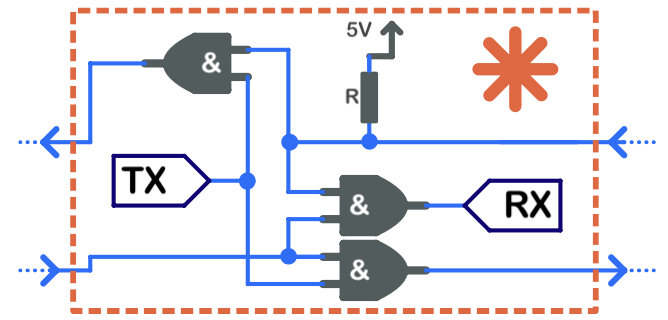
\includegraphics[width=0.28\textwidth]{Skripsie_LaTeXTemplate/Figures/BUS_CON.png}
\caption{Protection Logic Circuit}
\label{fig:buscon}
\end{figure}
\noindent
The final design equipped to each cell monitoring module is presented below in figure \ref{fig:klakom}, highlighted pathways represent the data flow of the communication system.

\begin{figure}[h!]
\centering
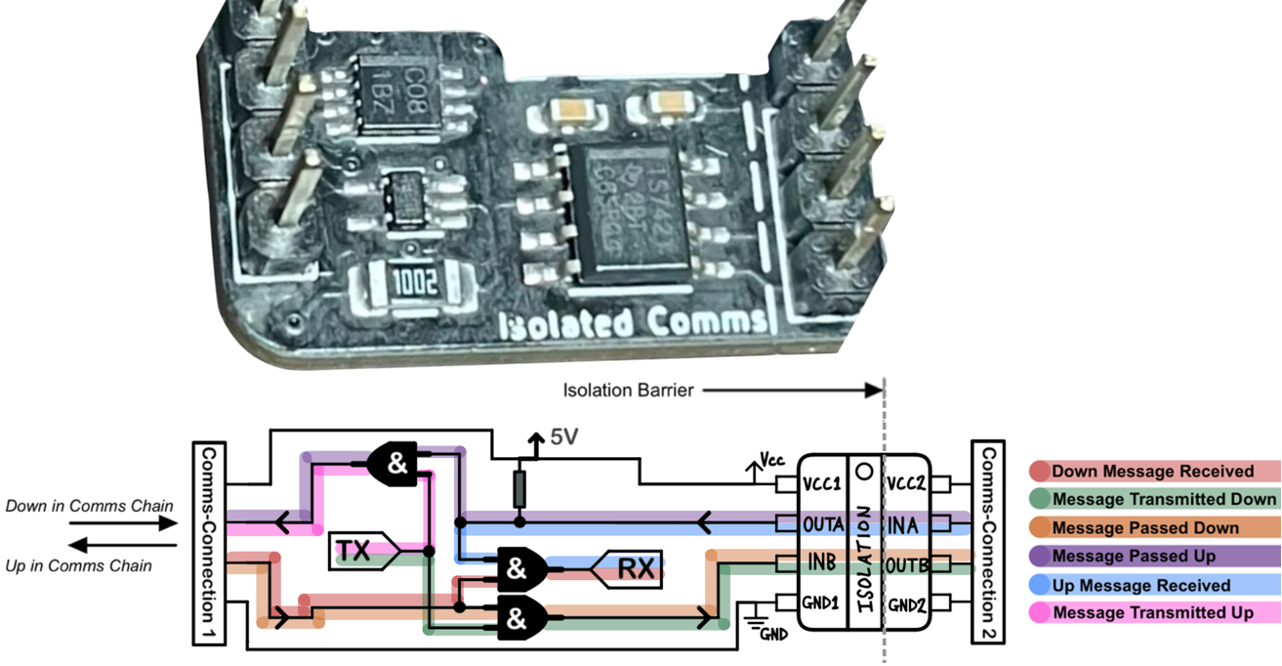
\includegraphics[width=0.75\textwidth]{Skripsie_LaTeXTemplate/Figures/FINAL_KOM.png}
\caption{Isolated Communication System Design}
\label{fig:klakom}
\end{figure}
%########################################################
\subsubsection{Printed Circuit Board Design}\label{subsec:mmmm3}
%########################################################
In the figure below, the left illustrates the PCB design encompassing all copper layers and component footprints selected during the design process of the cell monitoring module. Despite size constraints posing a challenge, the design, as depicted on the right, successfully accommodates a 3D representation of the module between the cell's terminals. Refer to Appendix \ref{appen:cad} for the complete CAD assembly design.

\begin{figure}[h!]
\centering
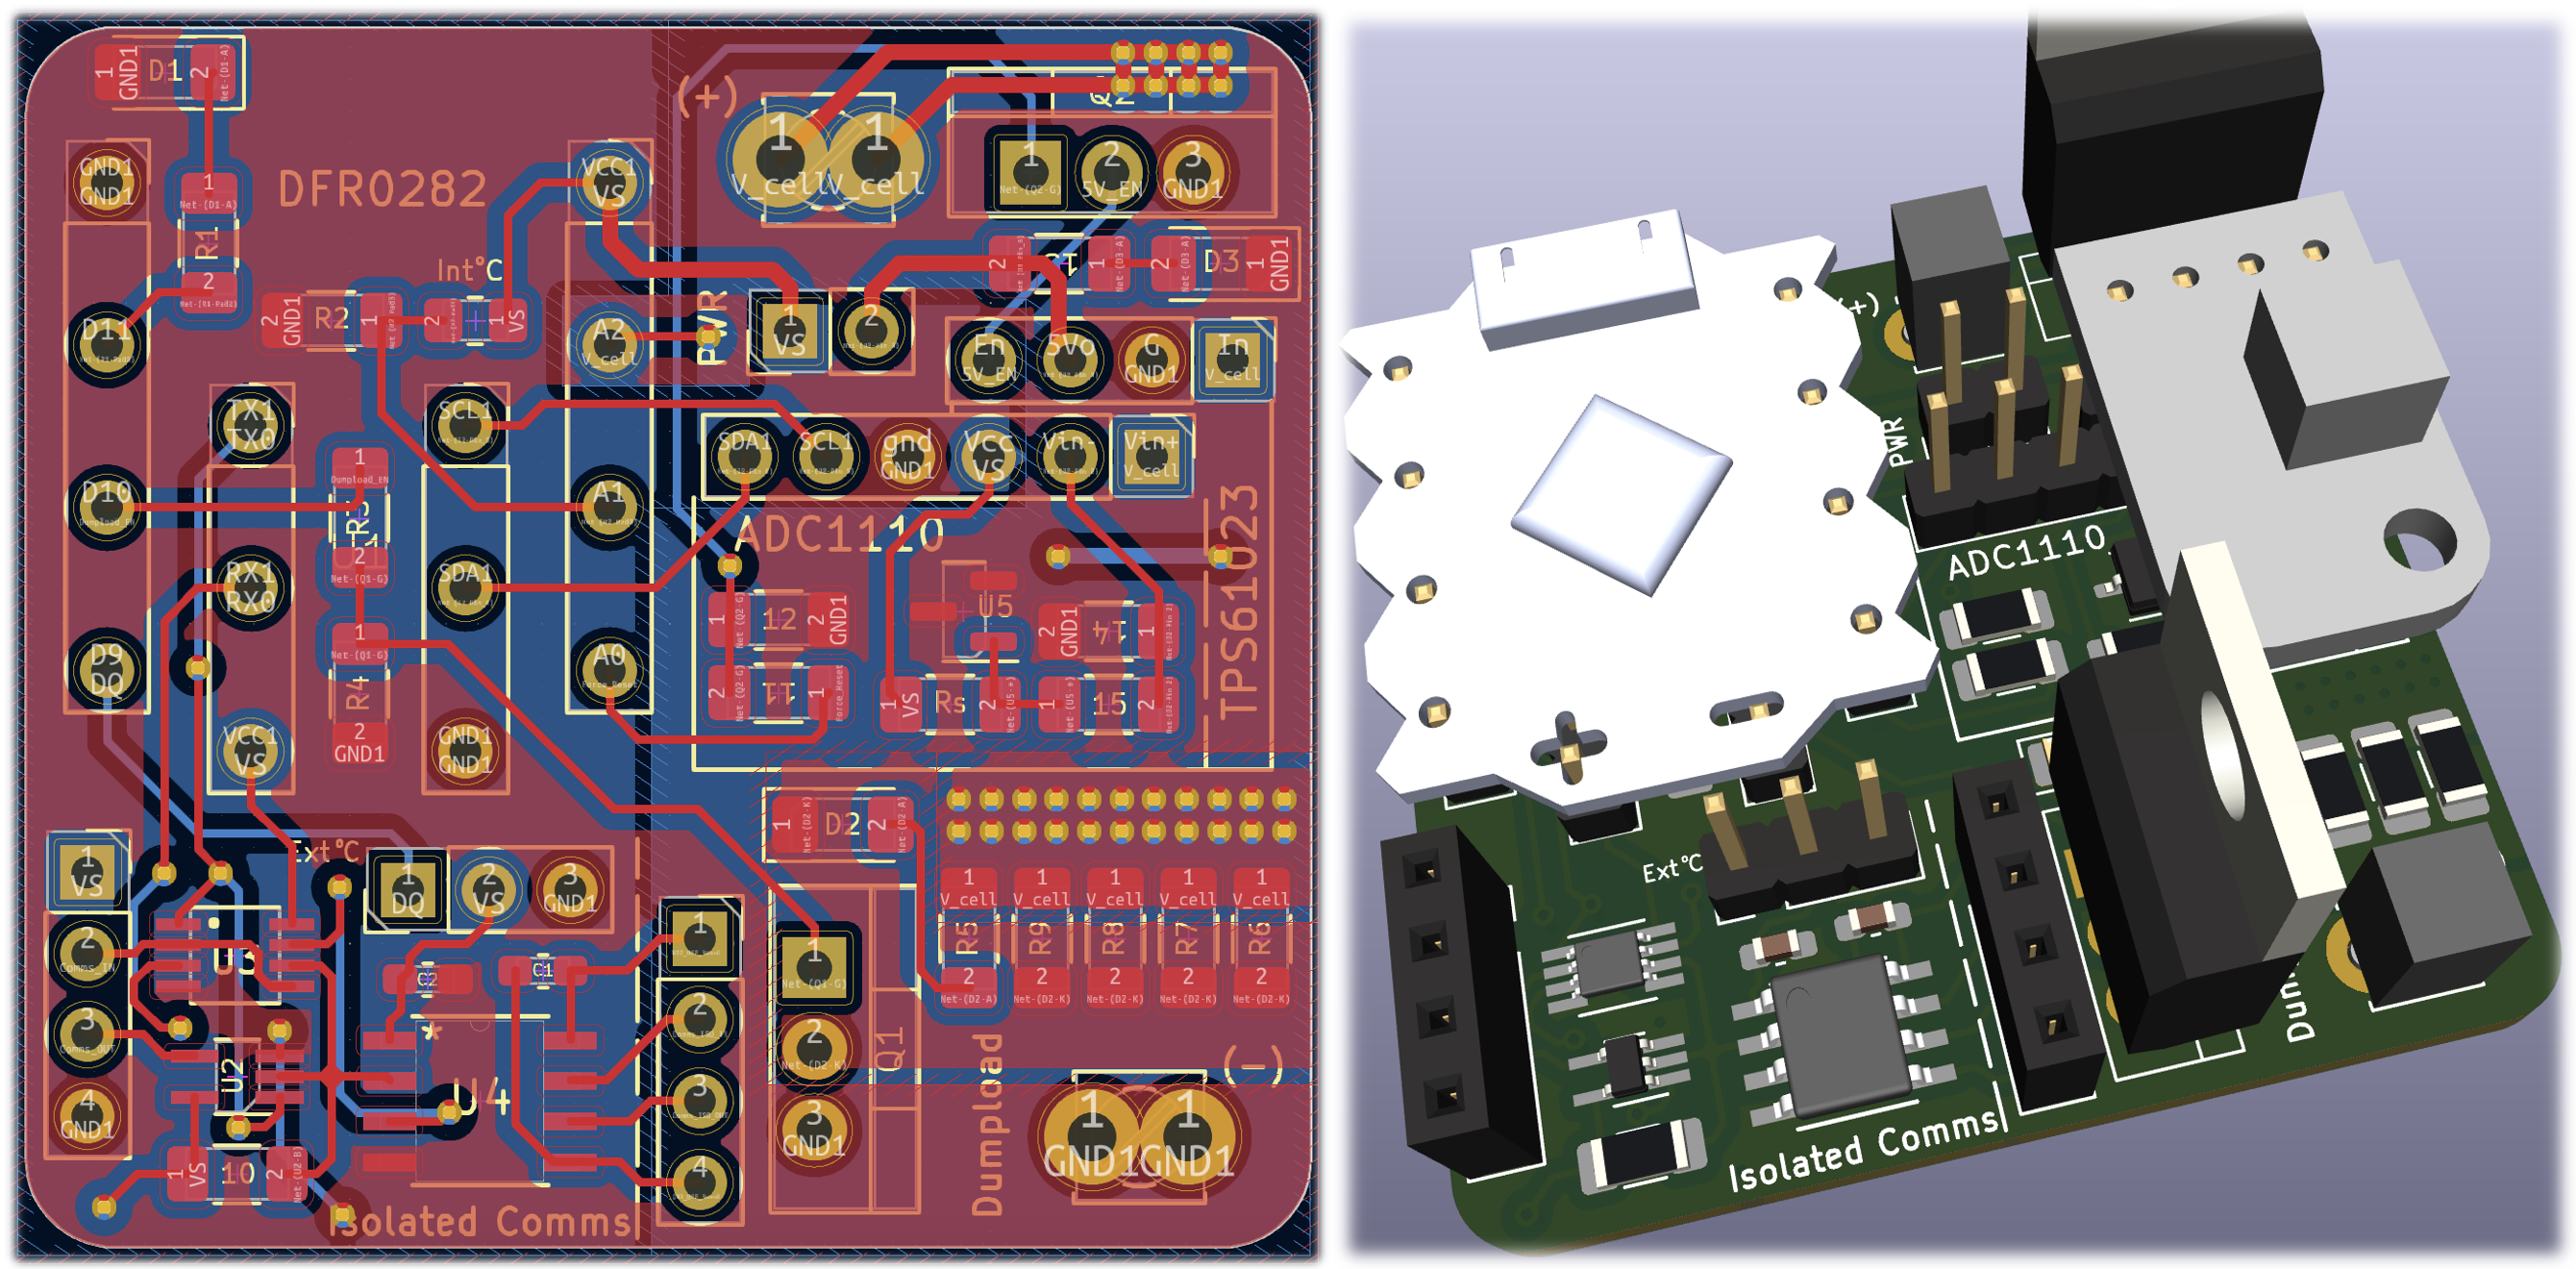
\includegraphics[width=0.77\textwidth]{Skripsie_LaTeXTemplate/Figures/MonitorPCB.png}
\caption{KiCad Software Monitoring Module Design \cite{ki}}
\label{fig:Monitoring_Board_PCB_2D}
\end{figure}
\newpage
%#####################################################################################################
\section{Master Controller Design}\label{subsec:mstr_contt}
%########################################################
\subsubsection{Design Outline}\label{subsec:mmmm4}
%########################################################
The main controller, serving as the master device in the communication system, solely monitors the current flowing into or out of the battery bank, while other battery parameters are relayed to it. It conducts real-time analysis to determine the connectivity of the battery to the load/charger, processes, and logs the data, primarily aiming to ensure battery safety and manage the state of cells within the battery bank. A meticulous inspection of the circuit design and component selection for each subsystem on the master controller board is delineated in the following section, with the PCB design further substantiating the system's compliance with the design requisites for power line control.

\begin{figure}[h!]
\centering
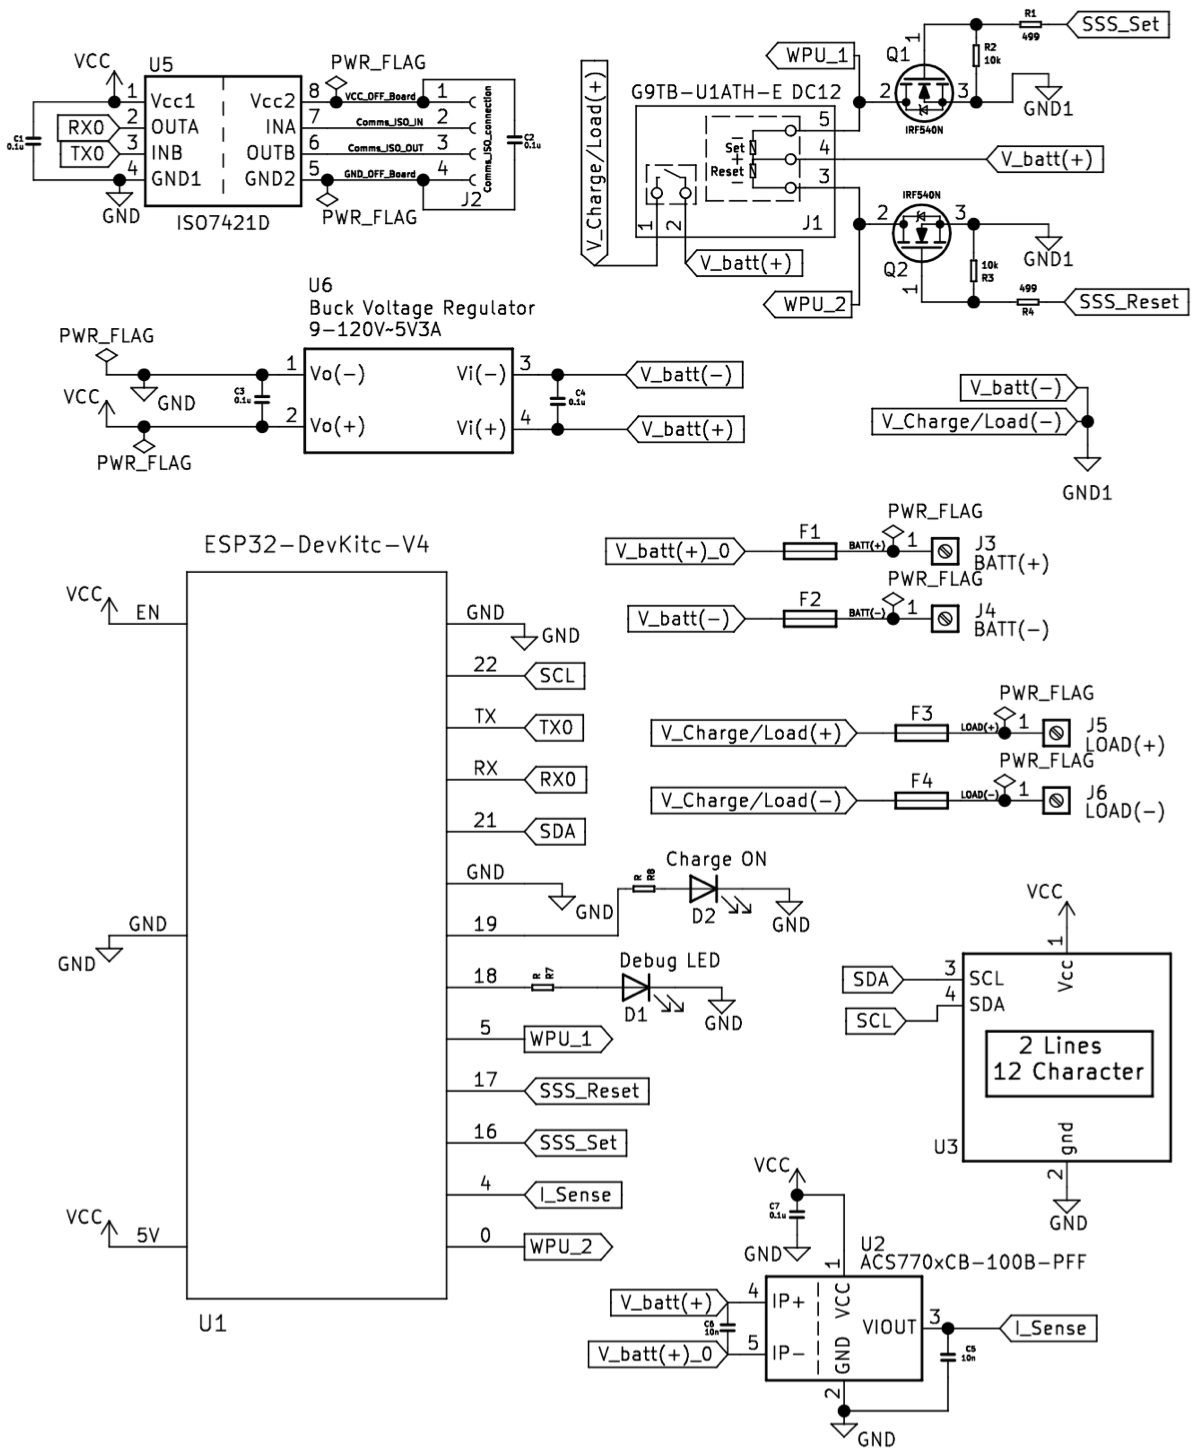
\includegraphics[width=0.82\textwidth]{Skripsie_LaTeXTemplate/Figures/Mstr_Schematic.png}
\caption{Main Controller Schematic Diagram}
\label{fig:Mstr_Schema}
\end{figure}
\newpage
%########################################################
\subsubsection{Circuit Designs \& Component Selection}\label{subsec:mmmm5}
%########################################################
\textbf{\emph{Terminals \& Fuse Protection}}\label{subsubsec:mstr_terminals_dsgn}

\begin{figure}[h!]
\centering
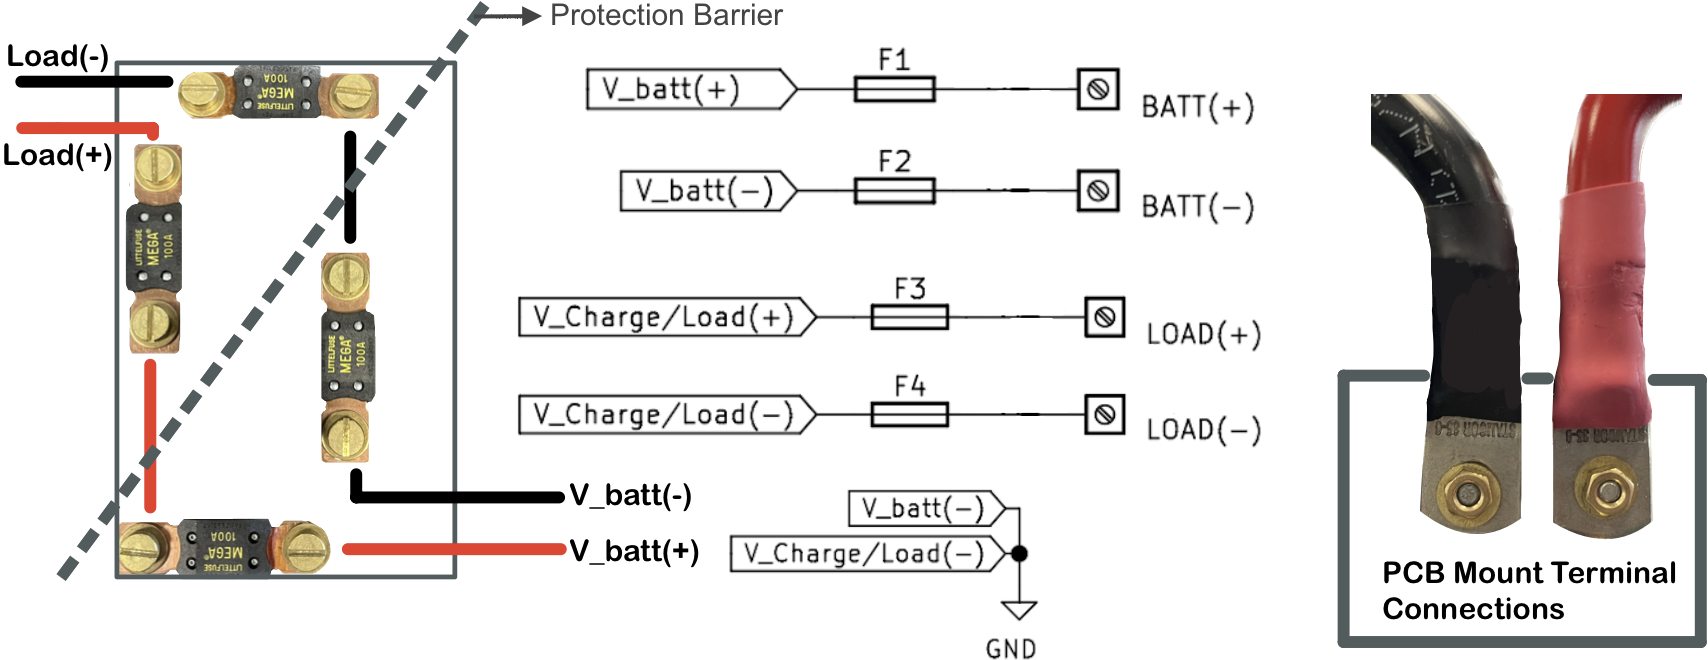
\includegraphics[width=0.7\textwidth]{Skripsie_LaTeXTemplate/Figures/Terminals_Fuses_DesigN.png}
\caption{Power Line Isolation \& Connections \cite{BigFuse}}
\label{fig:Mstr_D6}
\end{figure}
\noindent
Figure \ref{fig:Mstr_D6} illustrates the interconnection of the positive and negative lines of a battery pack and a load/charger via 130A PCB mount through hole screw terminals from Würth Elektronik \cite{BigTerminal}. To enhance safety, the controller employs 100A fuses \cite{BigFuse} on both lines, achieving complete isolation between the battery pack and the load/charger. This dual fusing strategy is essential in high voltage DC systems for mitigating risks associated with insulation failure that could lead to line-to-line DC short-circuit fault conditions. In a controlled setup like this power line control board, such fusing on both sides of the circuit safeguards the system against overcurrent conditions, thereby bolstering the reliability and safety of the control system. The incorporation of 100A fuses on both lines aligns with the best practices in high voltage DC system design, demonstrating a diligent approach to safety and protection.\newline\newline
%########################################################
\noindent
\textbf{\emph{Power Supply}}\label{subsubsec:mstr_Supp}\newline
\noindent
The choice of employing the Buck Voltage Regulator VIN 9-120V VOUT 5V3A \cite{12Vto5V} is dictated by the necessity for a stable 5V reference to power the control circuitry on the master board, similar to the monitoring module. For high scalability in the battery pack, this regulator provides a voltage range of 9V to 120V. This regulator not only caters to the maximum current demand of the system but also offers a surplus, ensuring a reliable power supply. The 5V logic level derived from this regulator facilitates a high resolution range, crucial for achieving precision in measurement processing within the system.\newline

\begin{figure}[h!]
\centering
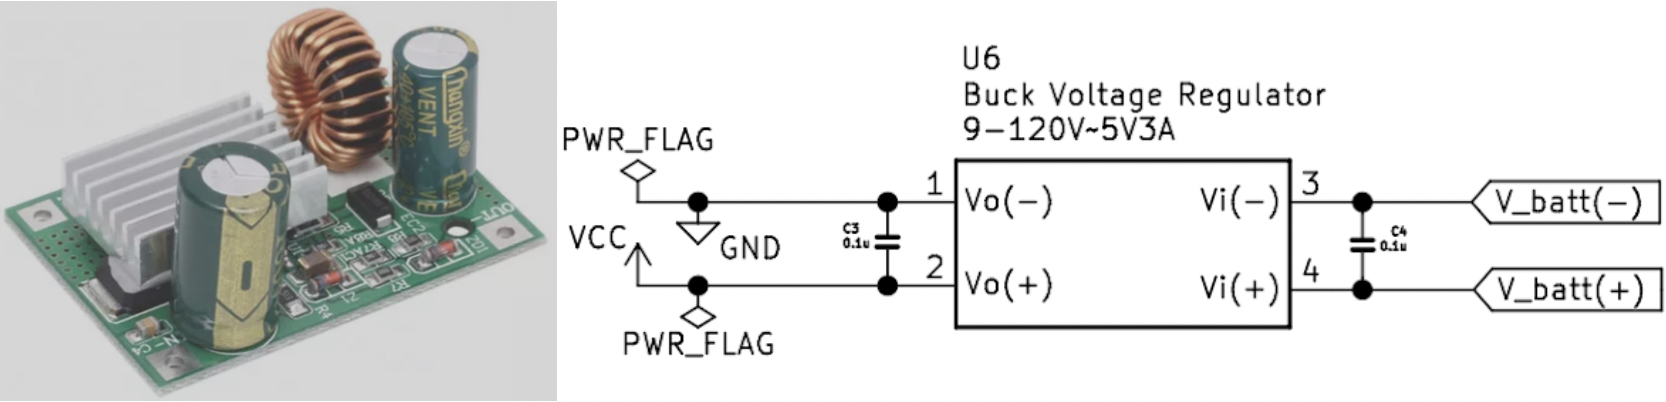
\includegraphics[width=0.7\textwidth]{Skripsie_LaTeXTemplate/Figures/P_Sup_DesigN.png}
\caption{Buck Voltage Regulator \cite{12Vto5V}}
\label{fig:Mstr_D5}
\end{figure}
\newpage
%########################################################
\noindent
\textbf{\emph{Master Microcontroller}}\label{subsubsec:ESP32_dsgn}\newline
\noindent
The ESP32 DevKitC V4 microcontroller by Espressif \cite{The_ESP_ref} is tailored for system controller applications, demonstrating adept handling of UART communication protocols for real-time interaction with slave monitoring devices. It processes data from series string cells efficiently and uploads it to the cloud via integrated Wi-Fi functionality, enabling real-time monitoring and system analysis.

\begin{figure}[h!]
\centering
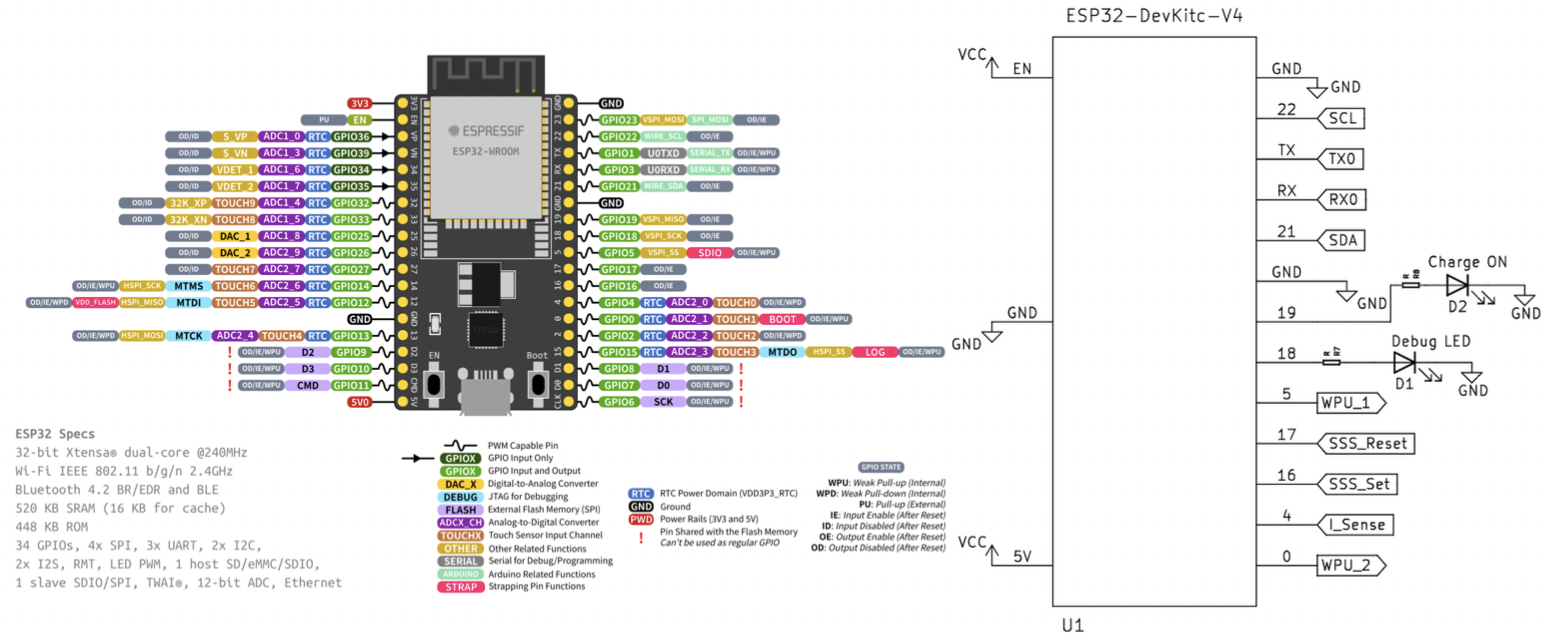
\includegraphics[width=1.0\textwidth]{Skripsie_LaTeXTemplate/Figures/The_ESP_DesigN.png}
\caption{ESP32DevKitCv4 Master Microcontroller \cite{The_ESP_ref}}
\label{fig:Mstr_D4}
\end{figure}
\noindent
This microcontroller is cost-effective compared to alternatives like the Raspberry Pi, yet provides a rich feature set. The on-board Wi-Fi ensures real-time data transmission and remote monitoring. Its compatibility with Arduino IDE facilitates effortless interfacing with DFR0282 slave modules for cell monitoring, simplifying development and accelerating deployment of monitoring and control logic. The ESP32 DevKitC V4 is mounted on the master controller board, featuring an on-board micro-USB port for program updates. Below is a table detailing the pin configurations and utilities on the master controller board.

\begin{table}[h]
    \centering
    \caption{Master Microcontroller Pin Out}
    \label{tab:ESP_PinOut}
    \begin{tabular}{|c|c|c|c|}
        \hline
        \textbf{ESP32-Pin} & \textbf{Name} & \textbf{Configuration} & \textbf{Utility} \\
        \hline
        \hline
        3 & IO22 & Arduino Wire-Lib SCL & I2C clock for LCD \\
        \hline
        4 & TX & UART Protocol & Serial transmit channel \\
        \hline
        5 & RX & UART Protocol & Serial recieve channel \\
        \hline
        6 & IO21 & Arduino Wire-Lib SDA & I2C data for LCD \\
        \hline
        8 & IO19 & Digital Output & Charge/Load ON indication \\
        \hline
        9 & IO18 & PWM Channel & System debug messages LED \\
        \hline
        10 & IO5 & GPIO State & Internal weak pull-up 1 \\
        \hline
        11 & IO17 & Digital Pulse & Lacthing relay RESET \\
        \hline
        12 & IO16 & Digital Pulse & Lacthing relay SET \\
        \hline
        13 & IO4 & Analog Channel & Current sensor input \\
        \hline
        14 & IO0 & GPIO State & Internal weak pull-up 2 \\
        \hline
    \end{tabular}
\end{table}
\newpage
%########################################################
\noindent
\textbf{\emph{Battery Current Measurement}}\label{subsubsec:cur_sen_design}\newline
\noindent
The ACS770LCB-100B current sensor from Allegro Microsystems \cite{currentSensori} is utilized to measure the current flowing from the battery's positive terminal to the load/charger. Accompanying the sensor are a $0.1 \mu F$ decoupling capacitor between its 5V supply lines, a $10 nF$ bypass capacitor at its output, and another $10 nF$ capacitor between the current path's positive and negative terminals for noise mitigation. The sensor's output delivers a voltage signal representative of the battery pack's current to the microcontroller, within a measurement range of -100A to 100A and a corresponding output voltage range of 0V to 5V.\newline\newline
\noindent
The linear transfer characteristic of the sensor is given by the formula below.
\[ V_{out} = V_{zero} + (S \cdot I) \]
\noindent
Where \(V_{zero} = 2.5V\) (sensor output at zero current) and \(S\) the sensitivity, is calculated.
\[ S = \frac{5V}{200A} = 0.025 \, \text{V/A} \]
\noindent
The accuracy of the measurement is evaluated considering a sensor accuracy specification of $0.5\%$. For a measured current of $50A$, the error and its corresponding voltage error are calculated as follows:
\begin{equation}
\label{eq:I_error}
\text{Error} = 0.5\% \cdot 50A = 0.25A
\end{equation}
\begin{equation}
\label{eq:V_error}
V_{\text{error}} = 0.025 \, \text{V/A} \cdot 0.25A = 0.00625V
\end{equation}

\begin{table}[h]
    \centering
    \caption{Sensor Voltage Output for Various Current Values}
    \label{tab:Sensor_Output}
    \begin{tabular}{|c|c|c|}
        \hline
        \textbf{Current (\(I\))} & \textbf{Expression} & \textbf{Output Voltage (\(V_{out}\))} \\
        \hline
        50A & \(2.5V + (0.025 \, \text{V/A} \cdot 50A)\) & 3.75V \\
        \hline
        -50A & \(2.5V + (0.025 \, \text{V/A} \cdot -50A)\) & 1.25V \\
        \hline
        100A & \(2.5V + (0.025 \, \text{V/A} \cdot 100A)\) & 5V \\
        \hline
    \end{tabular}
\end{table}

\noindent
The design, shown in figure \ref{fig:Mstr_D1}, leverages the ACS770LCB-100B to translate battery current to a voltage signal for microcontroller interpretation, with capacitors employed for noise suppression, thus bolstering system reliability and measurement accuracy.

\begin{figure}[h!]
\centering
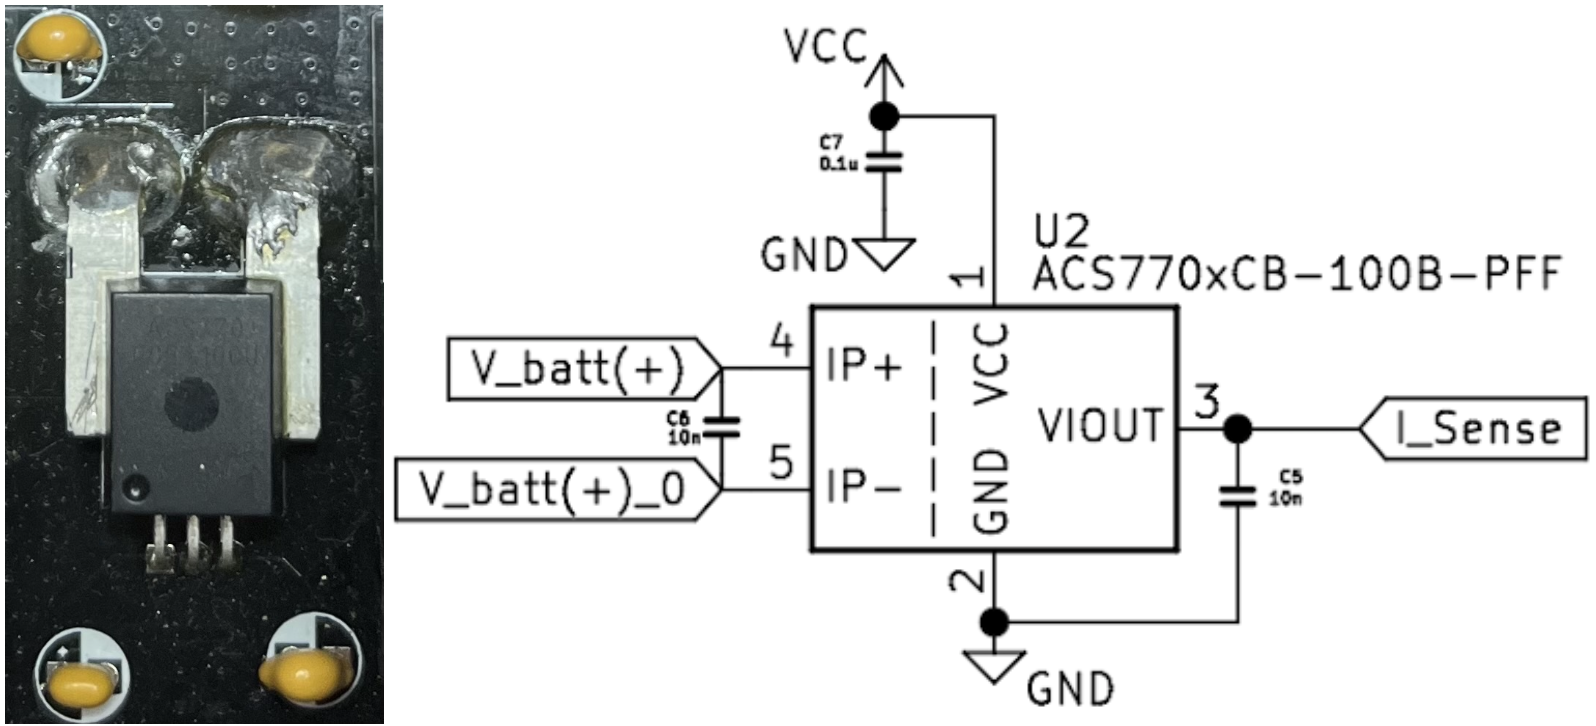
\includegraphics[width=0.5\textwidth]{Skripsie_LaTeXTemplate/Figures/Cur_Sen_DesigN.png}
\caption{Battery Cerrent Sensor \cite{currentSensori}}
\label{fig:Mstr_D1}
\end{figure}
\newpage
%########################################################
\noindent
\textbf{\emph{System Information Display}}\label{subsubsec:LCD_Dsgn}\newline
\noindent
The generic LCD 16x2 Character Display, White on Blue Background, 5V, along with the I2C Interface Module for LCD, 3.3/5V Ready, from Microrobotics \cite{LCD_MR}, are integrated on the control board. This setup facilitates communication between the microcontroller and the LCD via the I2C protocol. The I2C Interface Module simplifies the connection requiring only four wires: VCC, GND, SDA, and SCL. Through this setup, the microcontroller can dispatch summarized system messages to the LCD, providing a succinct insight into the state of system variables, ensuring a user-friendly interface for real-time system monitoring.

\begin{figure}[h!]
\centering
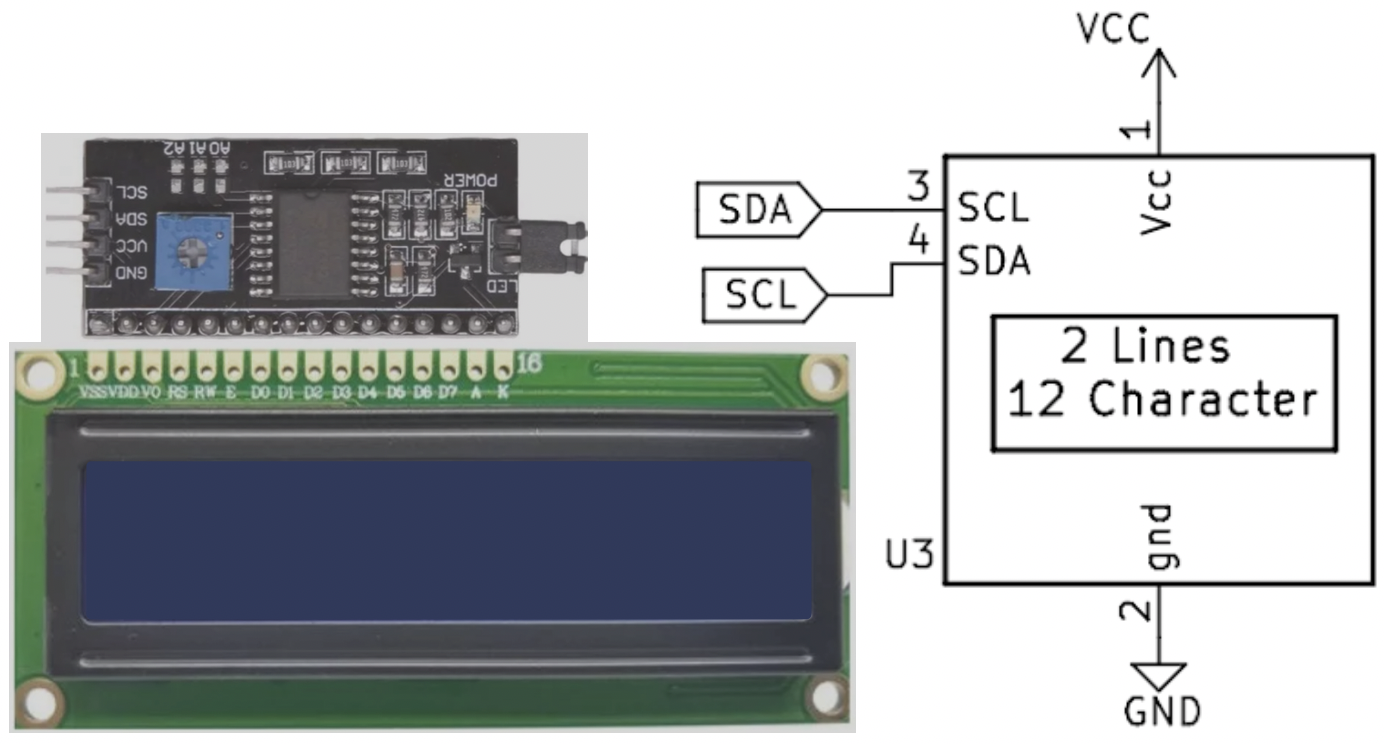
\includegraphics[width=0.36\textwidth]{Skripsie_LaTeXTemplate/Figures/The_LCD_DesigN.png}
\caption{LCD with I2C Module \cite{LCD_MR}}
\label{fig:Mstr_D3}
\end{figure}
%########################################################
\noindent
\textbf{\emph{Load/Charge Disconnect}}\label{subsubsec:relay_Dsgn}\newline
\noindent
The Omron G9TB-K1ATH-E DC12 relay, positioned in series between the battery pack and the load/charger, serves as a switch for power flow, safeguarded by fuse protection on both sides for a maximum current of 100A.

\begin{figure}[h!]
\centering
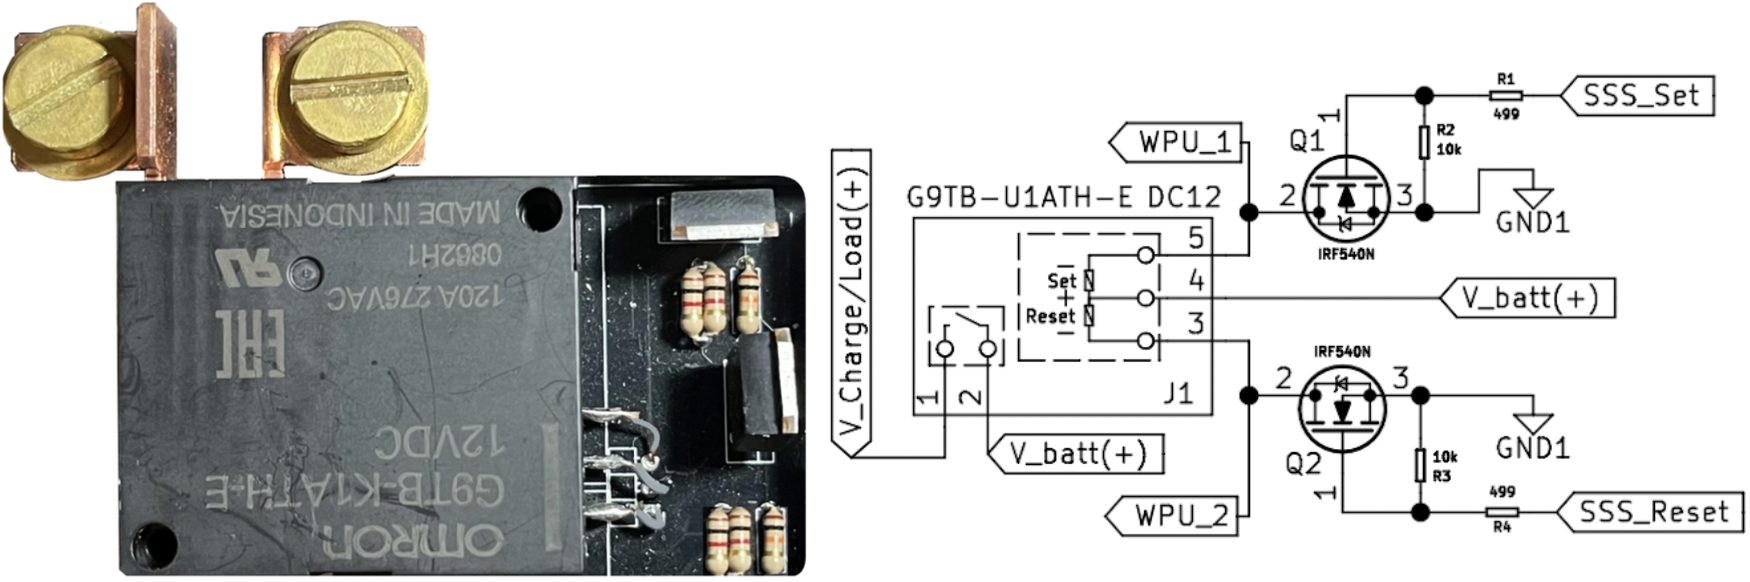
\includegraphics[width=0.7\textwidth]{Skripsie_LaTeXTemplate/Figures/Relay_DesigN.png}
\caption{Latching Power Relay \cite{RELAY}}
\label{fig:Mstr_D7}
\end{figure}
\noindent
The relay requires a 12V amplitude pulse for state transition, yet the ESP32 microcontroller outputs a maximum amplitude pulse of 5V. To bridge this voltage gap, external circuitry, depicted in figure \ref{fig:Mstr_D7}, is designed. Two identical MOSFETs from the dump-load circuits of the cell monitoring modules are integrated in low-side switch configurations, simplifying the design for gate limiting and pull-down resistors as per subsubsection \ref{subsubsec:LS_SW}.\newline\newline
\noindent
The gates of these MOSFETs are connected to distinct microcontroller pins labeled SET and RESET, enabling a 25ms pulse for the relay's operation. The common pin of the relay coils is tied to the positive battery voltage (12V), while the set and reset pins on the relay are linked to a MOSFET's drain pin and an internal pull-up pin of the microcontroller, ensuring the relay pins float high when MOSFETs are non-conductive.\newline\newline
\noindent
The source pins of each MOSFET are connected to the negative battery voltage (0V), enabling a 12V potential across the relay's set or reset coil upon a 5V, 25ms pulse from the microcontroller. A hardcoded protocol in the microcontroller ensures that SET and RESET pins are not pulsed concurrently, preventing erroneous relay actuations.
\newline\newline
%########################################################
\noindent
\textbf{\emph{Scalable Isolated Communication}}\label{subsubsec:iso_COMS_Mstr}

\begin{figure}[h!]
\centering
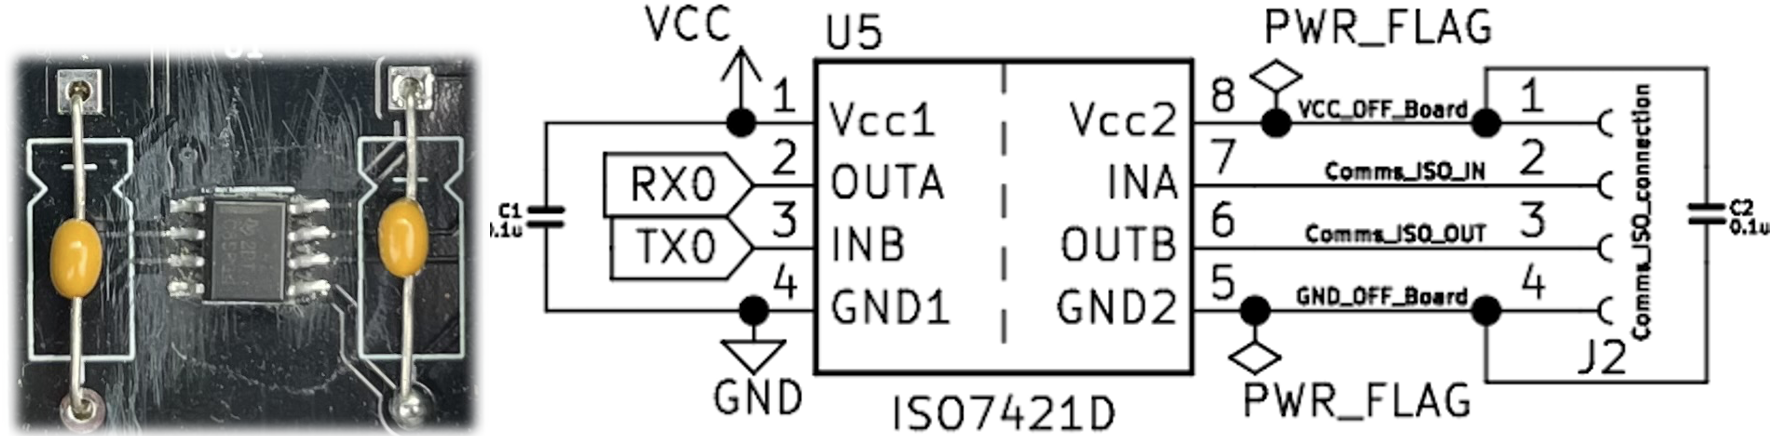
\includegraphics[width=0.4\textwidth]{Skripsie_LaTeXTemplate/Figures/Mstr_Comms_DesigN.png}
\caption{Master Controller Isolated Communication}
\label{fig:Mstr_D2}
\end{figure}
\noindent
The master controller's communication lines are isolated using the ISO7421D chip, identical to the one used in the cell monitoring modules as referenced in subsubsection \ref{subsubsec:iso_COMS}. Being at the start of the communication line, the master device is shielded against bus contention by the logic circuit on the first slave device in the stack.
%########################################################
\subsubsection{Printed Circuit Board Design}\label{subsec:mmmm6}
%########################################################
\begin{figure}[h!]
\centering
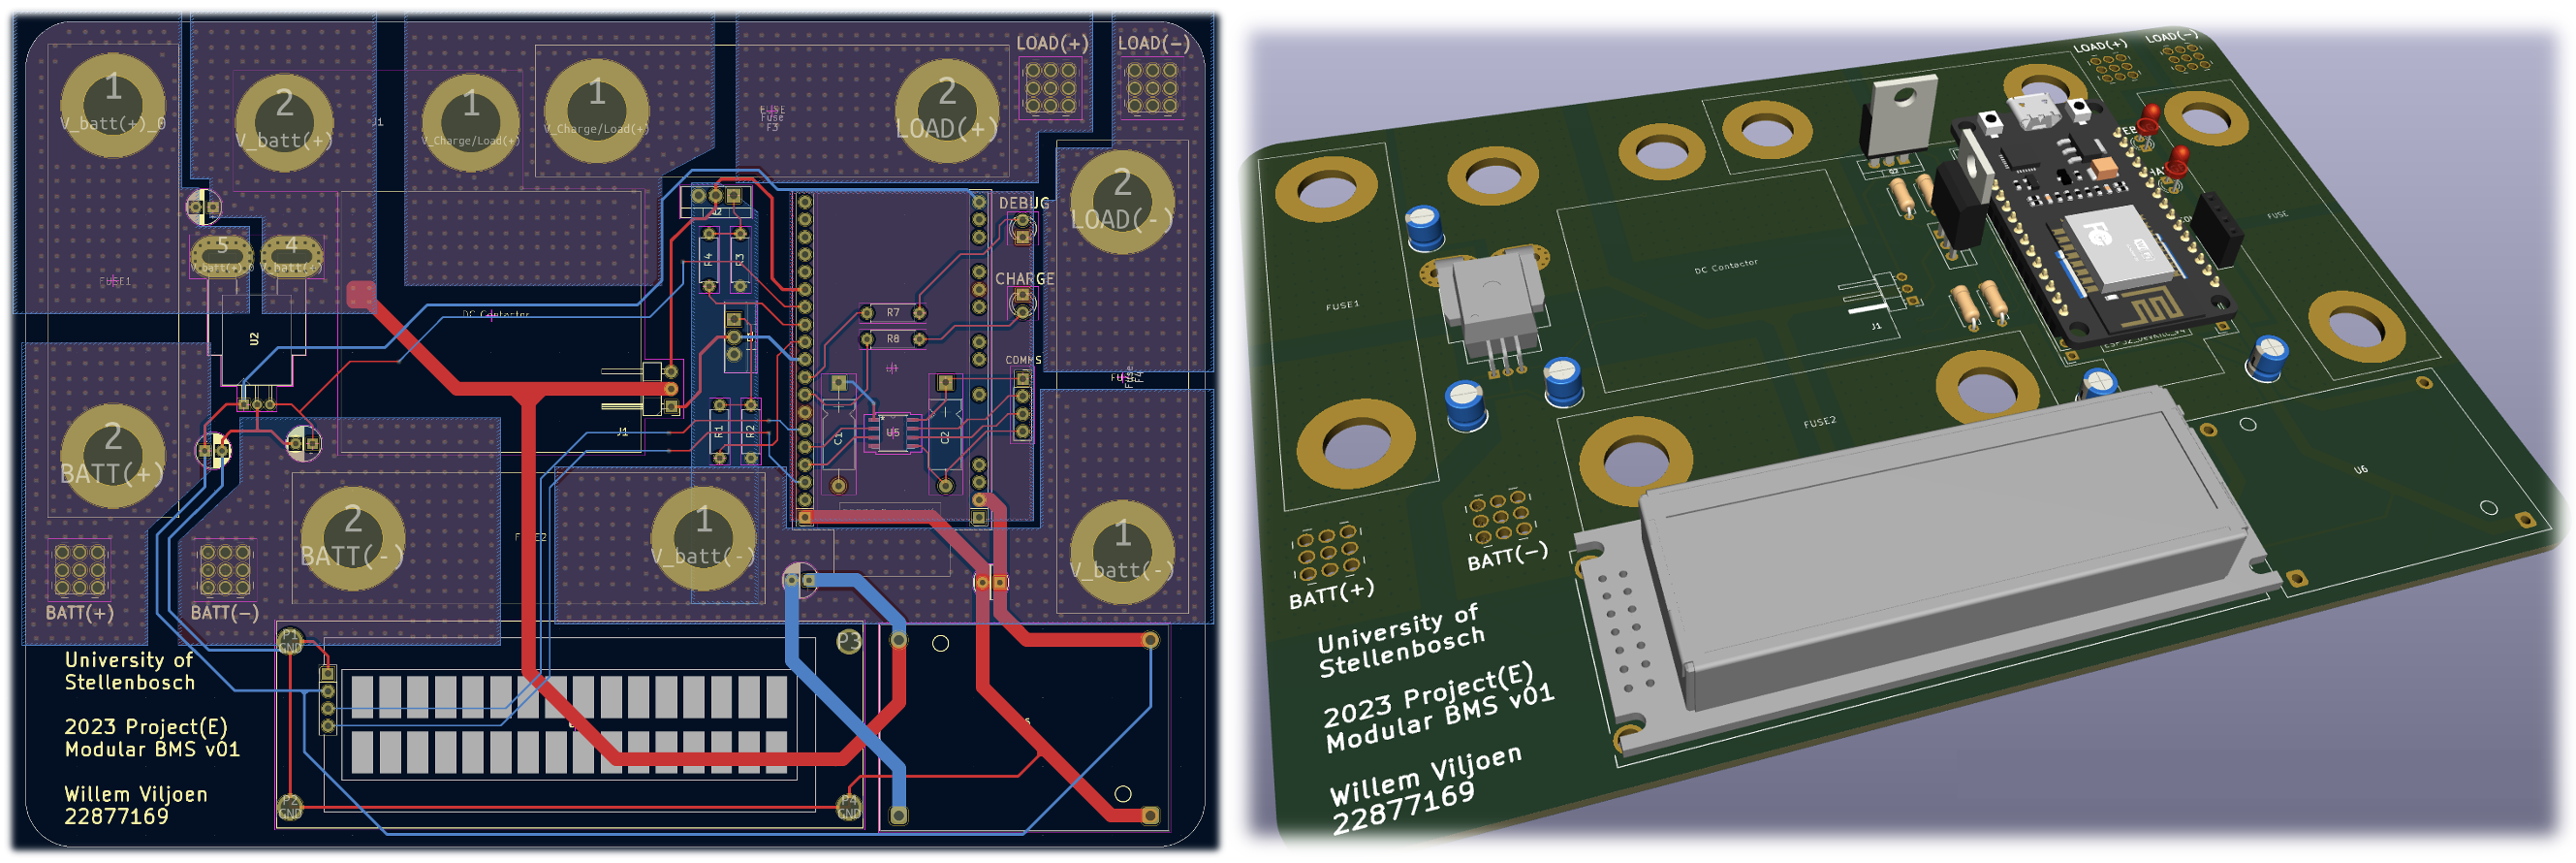
\includegraphics[width=0.94\textwidth]{Skripsie_LaTeXTemplate/Figures/ControllerPCB.png}
\caption{KiCad Software Master Controller Design}
\label{fig:Master_Board_PCB_2D}
\end{figure}
\noindent
In the figure above, the left illustrates the PCB design, showcasing all copper layers and component footprints selected during the design process of the master controller board. To accommodate a high current of 120A on the battery power lines flowing through the master controller board, filled copper layers and via stitching techniques were employed. These design approaches enhance the current-carrying capacity and thermal management of the PCB. A thermal test for the current capability of the master controller board is slated for evaluation in Section \ref{sec:systEVAL}. As depicted on the right, the design successfully integrates a 3D representation of the board, fitting perfectly to the side of the first cell in the series stack at the battery bank's input/output. Refer to Appendix \ref{appen:cad} for the complete CAD assembly design.
\newpage
%########################################################
\section{Design Review}\label{subsec:Des_Review}
%########################################################
The diagram below succinctly illustrates the system solution for \emph{a Modular Battery Management System for LFP Batteries}, showcasing the independent yet compatible monitoring modules and the master controller. These units, while autonomous, are interconnected through a communication network to form a cohesive BMS ecosystem for a battery bank. The design underscores the synergy between the controller, cell modules, and communication system, functioning both individually and collectively to ensure system integrity.

\begin{figure}[h!]
\centering
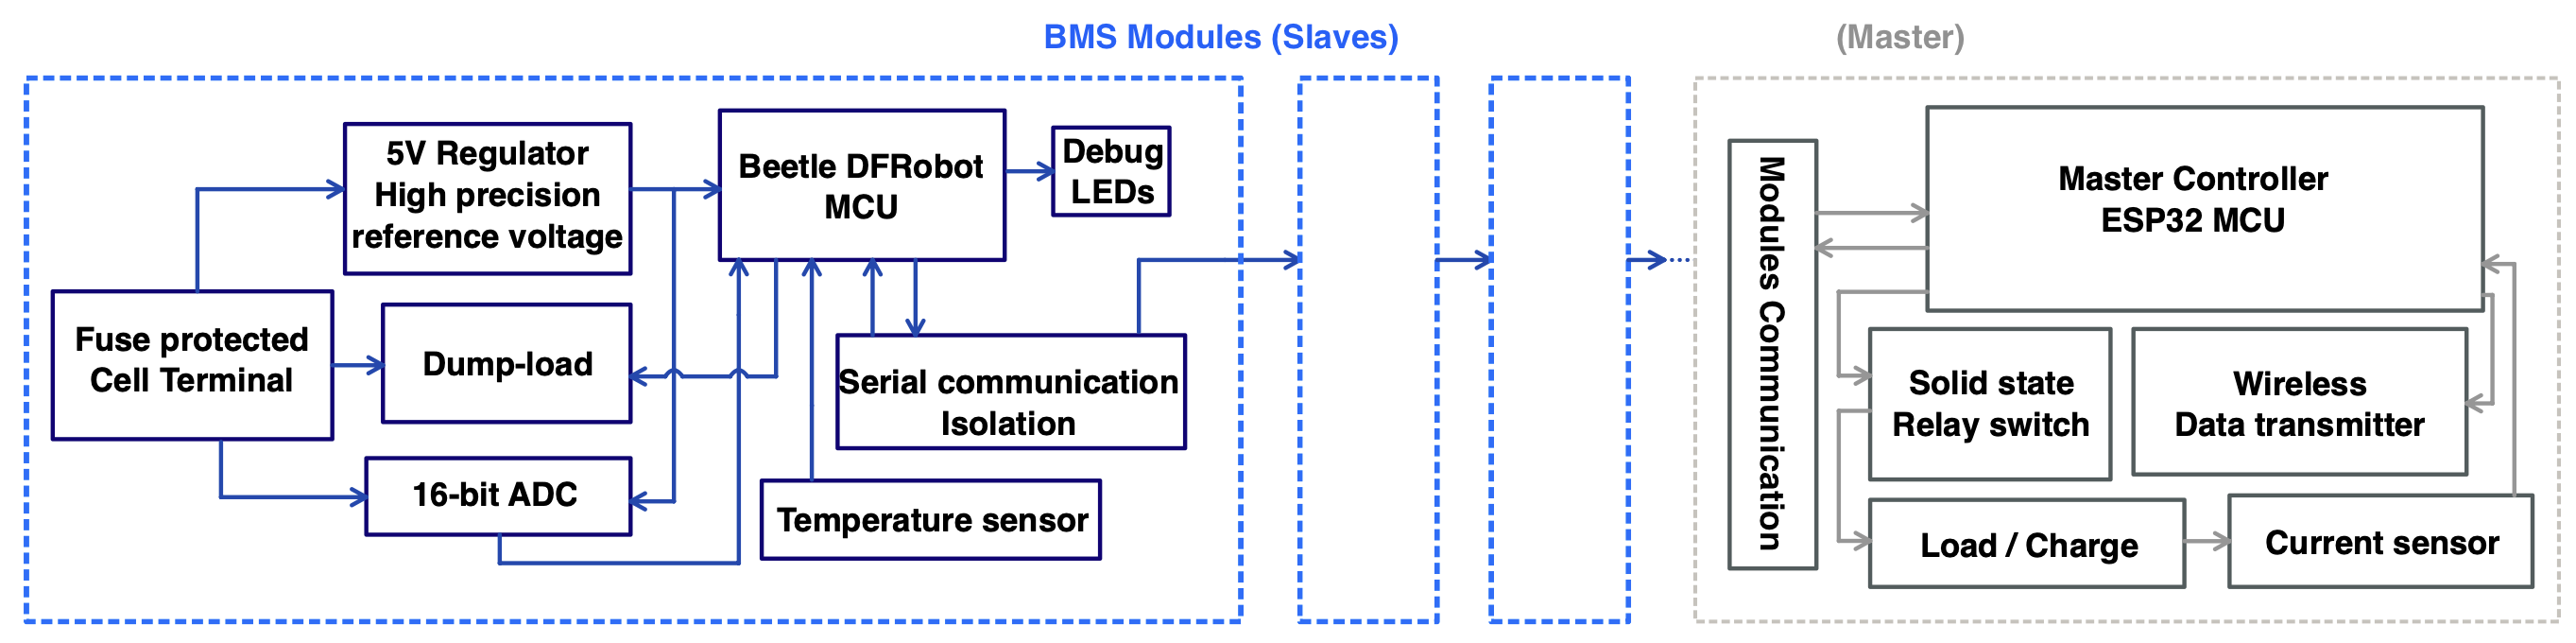
\includegraphics[width=1.0\textwidth]{Skripsie_LaTeXTemplate/Figures/setup.png}
\caption{Complete System Design}
\label{fig:setup_dsgn}
\end{figure}
\noindent
The modular BMS topology features cell-level monitoring modules and a central controller, marking a significant evolution in energy management. It achieves precise, real-time data collection and enhances system-wide awareness. Embedded microcontrollers within each module process data locally, reducing latency and improving accuracy, which simplifies the system's complexity and improves reliability.\newline\newline
\noindent
The central controller is pivotal, managing data flow and system communications with a focus on power control and resilient PCB design. It synthesizes cell data, supporting informed energy management decisions. In sum, the BMS melds modular design with centralized oversight, offering scalability and adaptability to meet evolving battery management needs, and is poised to set new industry benchmarks.\newline\newline
\noindent
\textbf{\emph{Design Tools Acknowledgment:}}\newline
\noindent
The subsequent figure presents a curated selection of icons representing the sophisticated design and development software applications instrumental to the engineering and design processes of this project.

\begin{figure}[h!]
\centering

\includegraphics[width=0.9\textwidth]{Skripsie_LaTeXTemplate/Figures/icons.png}
\caption{Design Software Packages}
\label{fig:DSP}
\end{figure}

\vfill
